%%%%%%%%%%%%%%%%%%%%%%%%%%%%%%%%%%%%%%%%%
% Beamer Presentation
% LaTeX Template
% Version 1.0 (10/11/12)
%
% This template has been downloaded from:
% http://www.LaTeXTemplates.com
%
% License:
% CC BY-NC-SA 3.0 (http://creativecommons.org/licenses/by-nc-sa/3.0/)
%
%%%%%%%%%%%%%%%%%%%%%%%%%%%%%%%%%%%%%%%%%

%----------------------------------------------------------------------------------------
%	PACKAGES AND THEMES
%----------------------------------------------------------------------------------------

\documentclass{beamer}

\mode<presentation> {

% The Beamer class comes with a number of default slide themes
% which change the colors and layouts of slides. Below this is a list
% of all the themes, uncomment each in turn to see what they look like.

%\usetheme{default}
%\usetheme{AnnArbor}
%\usetheme{Antibes}
%\usetheme{Bergen}
%\usetheme{Berkeley}
%\usetheme{Berlin}
%\usetheme{Boadilla}
%\usetheme{CambridgeUS}
%\usetheme{Copenhagen}
%\usetheme{Darmstadt}
%\usetheme{Dresden}
%\usetheme{Frankfurt}
%\usetheme{Goettingen}
%\usetheme{Hannover}
%\usetheme{Ilmenau}
%\usetheme{JuanLesPins}
%\usetheme{Luebeck}
%\usetheme{Madrid}
%\usetheme{Malmoe}
%\usetheme{Marburg}
%\usetheme{Montpellier}
%\usetheme{PaloAlto}
%\usetheme{Pittsburgh}
\usetheme{Rochester}
%\usetheme{Singapore}
%\usetheme{Szeged}
%\usetheme{Warsaw}

% As well as themes, the Beamer class has a number of color themes
% for any slide theme. Uncomment each of these in turn to see how it
% changes the colors of your current slide theme.

%\usecolortheme{albatross}
%\usecolortheme{beaver}
%\usecolortheme{beetle}
%\usecolortheme{crane}
%\usecolortheme{dolphin}
%\usecolortheme{dove}
%\usecolortheme{fly}
%\usecolortheme{lily}
%\usecolortheme{orchid}
%\usecolortheme{rose}
%\usecolortheme{seagull}
%\usecolortheme{seahorse}
%\usecolortheme{whale}
%\usecolortheme{wolverine}

%\setbeamertemplate{footline} % To remove the footer line in all slides uncomment this line
%\setbeamertemplate{footline}[page number] % To replace the footer line in all slides with a simple slide count uncomment this line

\setbeamertemplate{navigation symbols}{} % To remove the navigation symbols from the bottom of all slides uncomment this line

\definecolor{OUGold}{RGB}{181,154,57}
\setbeamercolor{structure}{fg=OUGold}
\setbeamercolor{block title example}{bg=OUGold}
\setbeamercolor{section in toc}{fg=black}

% position the logo
\addtobeamertemplate{frametitle}{}{%
	\begin{textblock*}{\paperwidth}(290pt,-38pt)
		
\includegraphics[height=1cm,keepaspectratio]{sail}
	\end{textblock*}}
}

\usepackage{textpos} % package for the positioning
\usepackage{graphicx} % Allows including images
\usepackage{booktabs} % Allows the use of \toprule, \midrule and \bottomrule in tables
\usepackage{pdfpages} % Allows including PDFs (in separate frame)

%----------------------------------------------------------------------------------------
%	TITLE PAGE
%----------------------------------------------------------------------------------------

\title[Text Mining Project]{Text Mining Project: Presentation 2} % The short title appears at the bottom of every slide, the full title is only on the title page

\author{Evan Bradley} % Your name
\institute[OU] % Your institution as it will appear on the bottom of every slide, may be shorthand to save space
{
Oakland University \\ % Your institution for the title page
\medskip
\textit{edbradley@oakland.edu} % Your email address
}
\date{November 2016} % Date, can be changed to a custom date

\begin{document}

\begin{frame}
	\frametitle{\space}
	\titlepage % Print the title page as the first slide
\end{frame}

\begin{frame}
\frametitle{Overview} % Table of contents slide, comment this block out to remove it
\tableofcontents % Throughout your presentation, if you choose to use \section{} and \subsection{} commands, these will automatically be printed on this slide as an overview of your presentation
\end{frame}

%----------------------------------------------------------------------------------------
%	PRESENTATION SLIDES
%----------------------------------------------------------------------------------------

%------------------------------------------------
\section{Overview of Data} % Sections can be created in order to organize your presentation into discrete blocks, all sections and subsections are automatically printed in the table of contents as an overview of the talk
%------------------------------------------------

%\subsection{Test} % A subsection can be created just before a set of slides with a common theme to further break down your presentation into chunks

%------------------------------------------------

% Collected data stats
% Collection and preprocessing with Node.js
% Analysis using R
% Already produced results
% Goals for analysis

\begin{frame}
	\frametitle{Hashtags}
	\begin{itemize}
		\item \#Election2016: 50,000 tweets
		\newline
		\item \#NotMyPresident: 150,000 tweets
		\newline
		\item \#ElectionNight: 50,000 tweets
		\newline
		\item \#ElectionFinalThoughts: 1,500 tweets
		\newline
	\end{itemize}
\end{frame}

\begin{frame}
	\frametitle{Preprocessing}
	\begin{itemize}
    \item Used node.js for most preprocessing.
    \newline
    \item Got rid of most of the data given by Twitter.
    \newline
    \item Kept: timestamp, emoji, hashtags, text, retweet, biography, and location.
    \newline
	\end{itemize}
\end{frame}

% ------------------------------------------------
\section{Analysis} % Sections can be created in order to organize your presentation into discrete blocks, all sections and subsections are automatically printed in the table of contents as an overview of the talk
%------------------------------------------------

\begin{frame}
	\frametitle{Number of Tweets Over Time (Election2016)}
  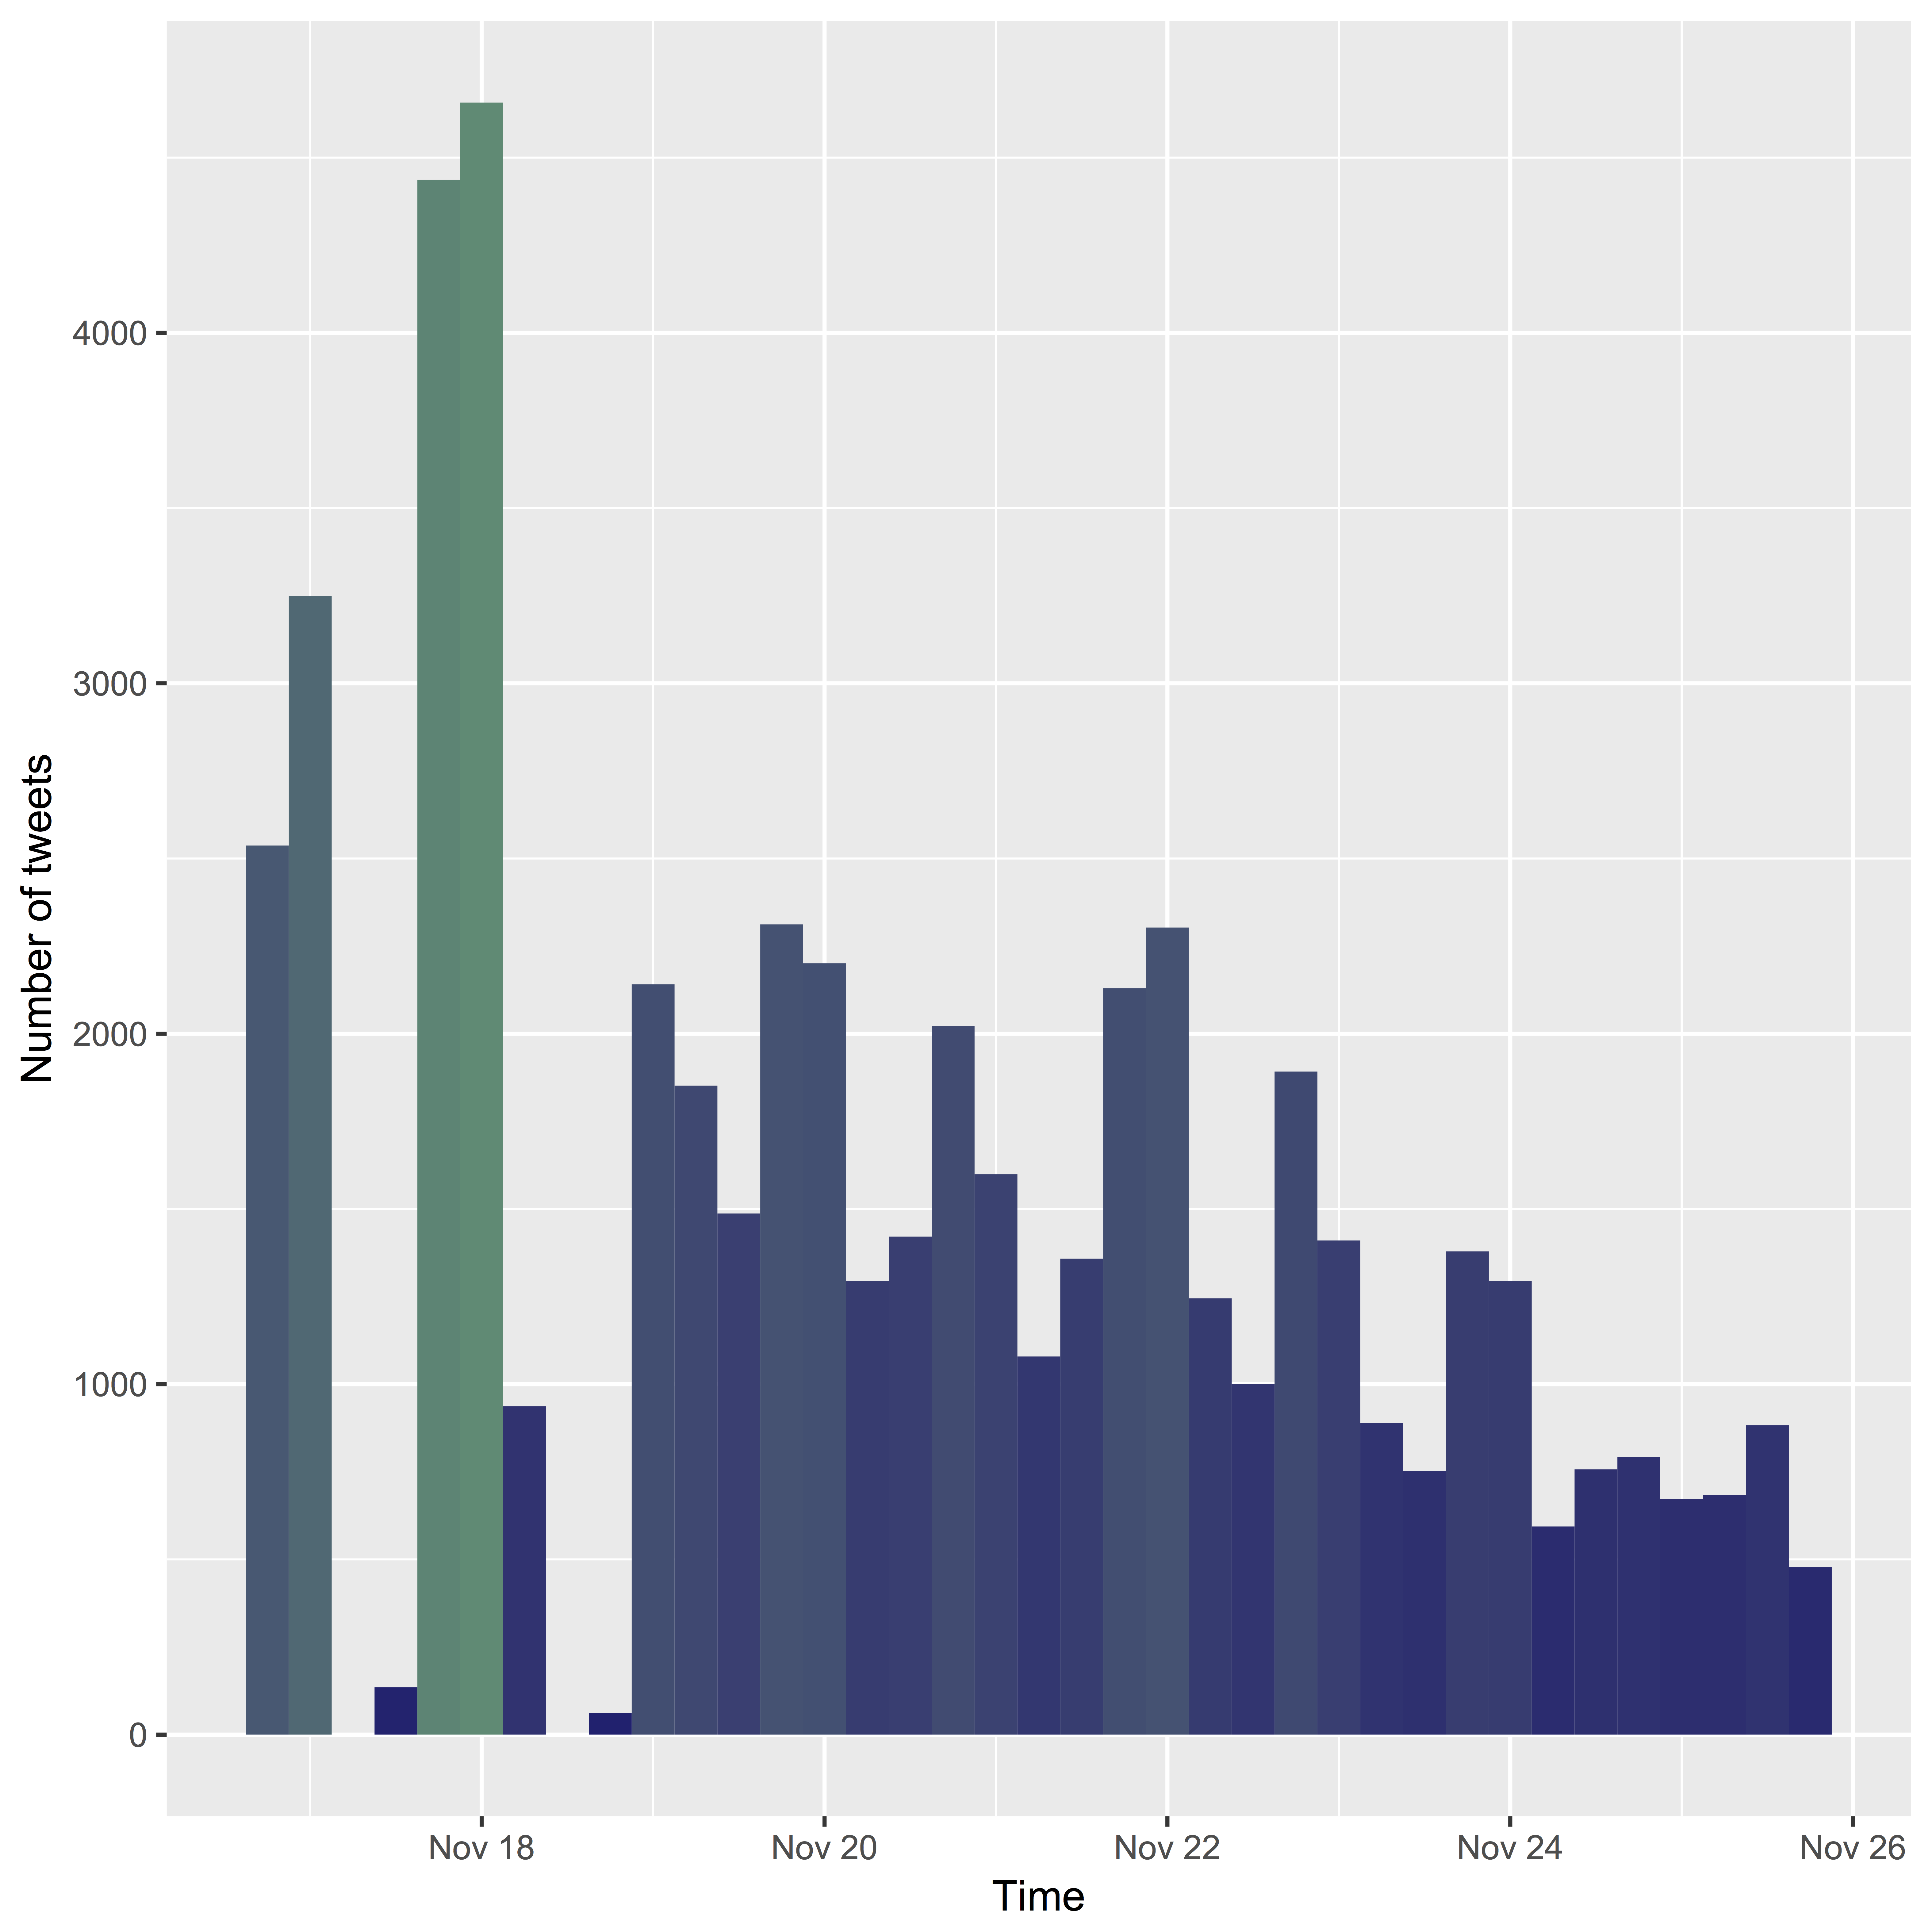
\includegraphics[height = 0.9\textheight]{e2016freq}
\end{frame}

\begin{frame}
	\frametitle{Number of Tweets Over Time (ElectionNight)}
  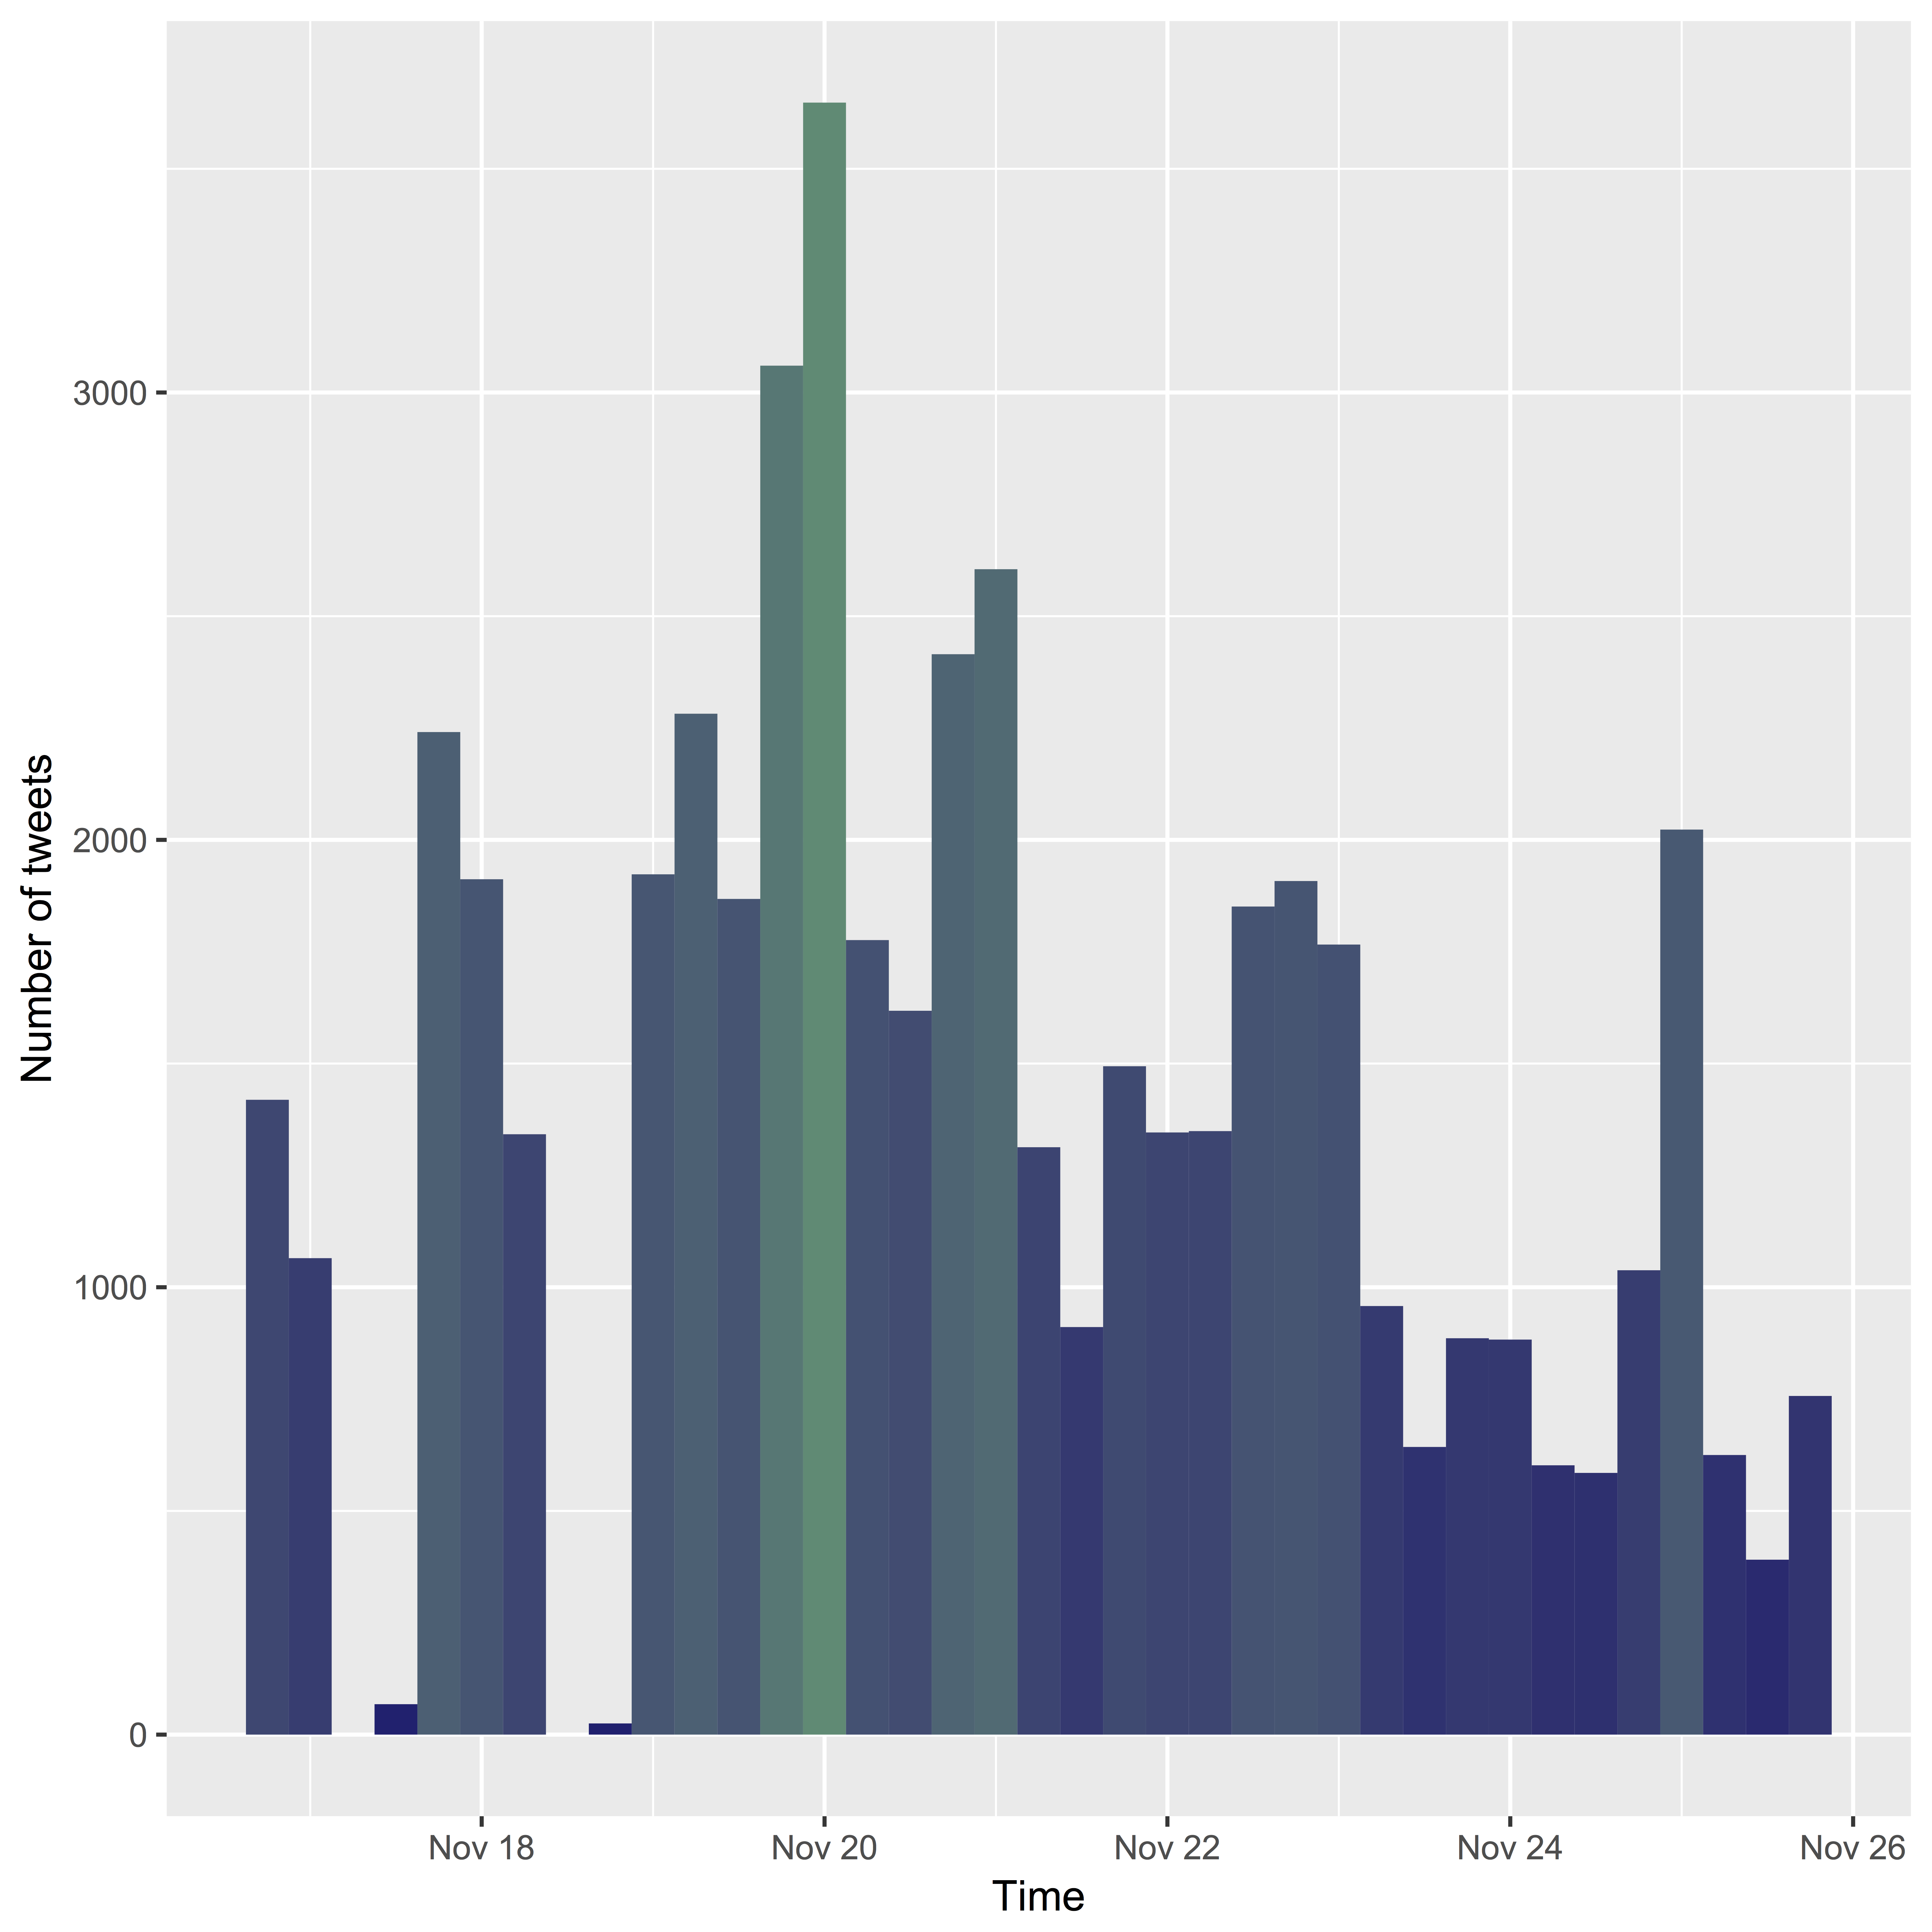
\includegraphics[height = 0.9\textheight]{enfreq}
\end{frame}

\begin{frame}
	\frametitle{Number of Tweets Over Time (ElectionFinalThoughts)}
  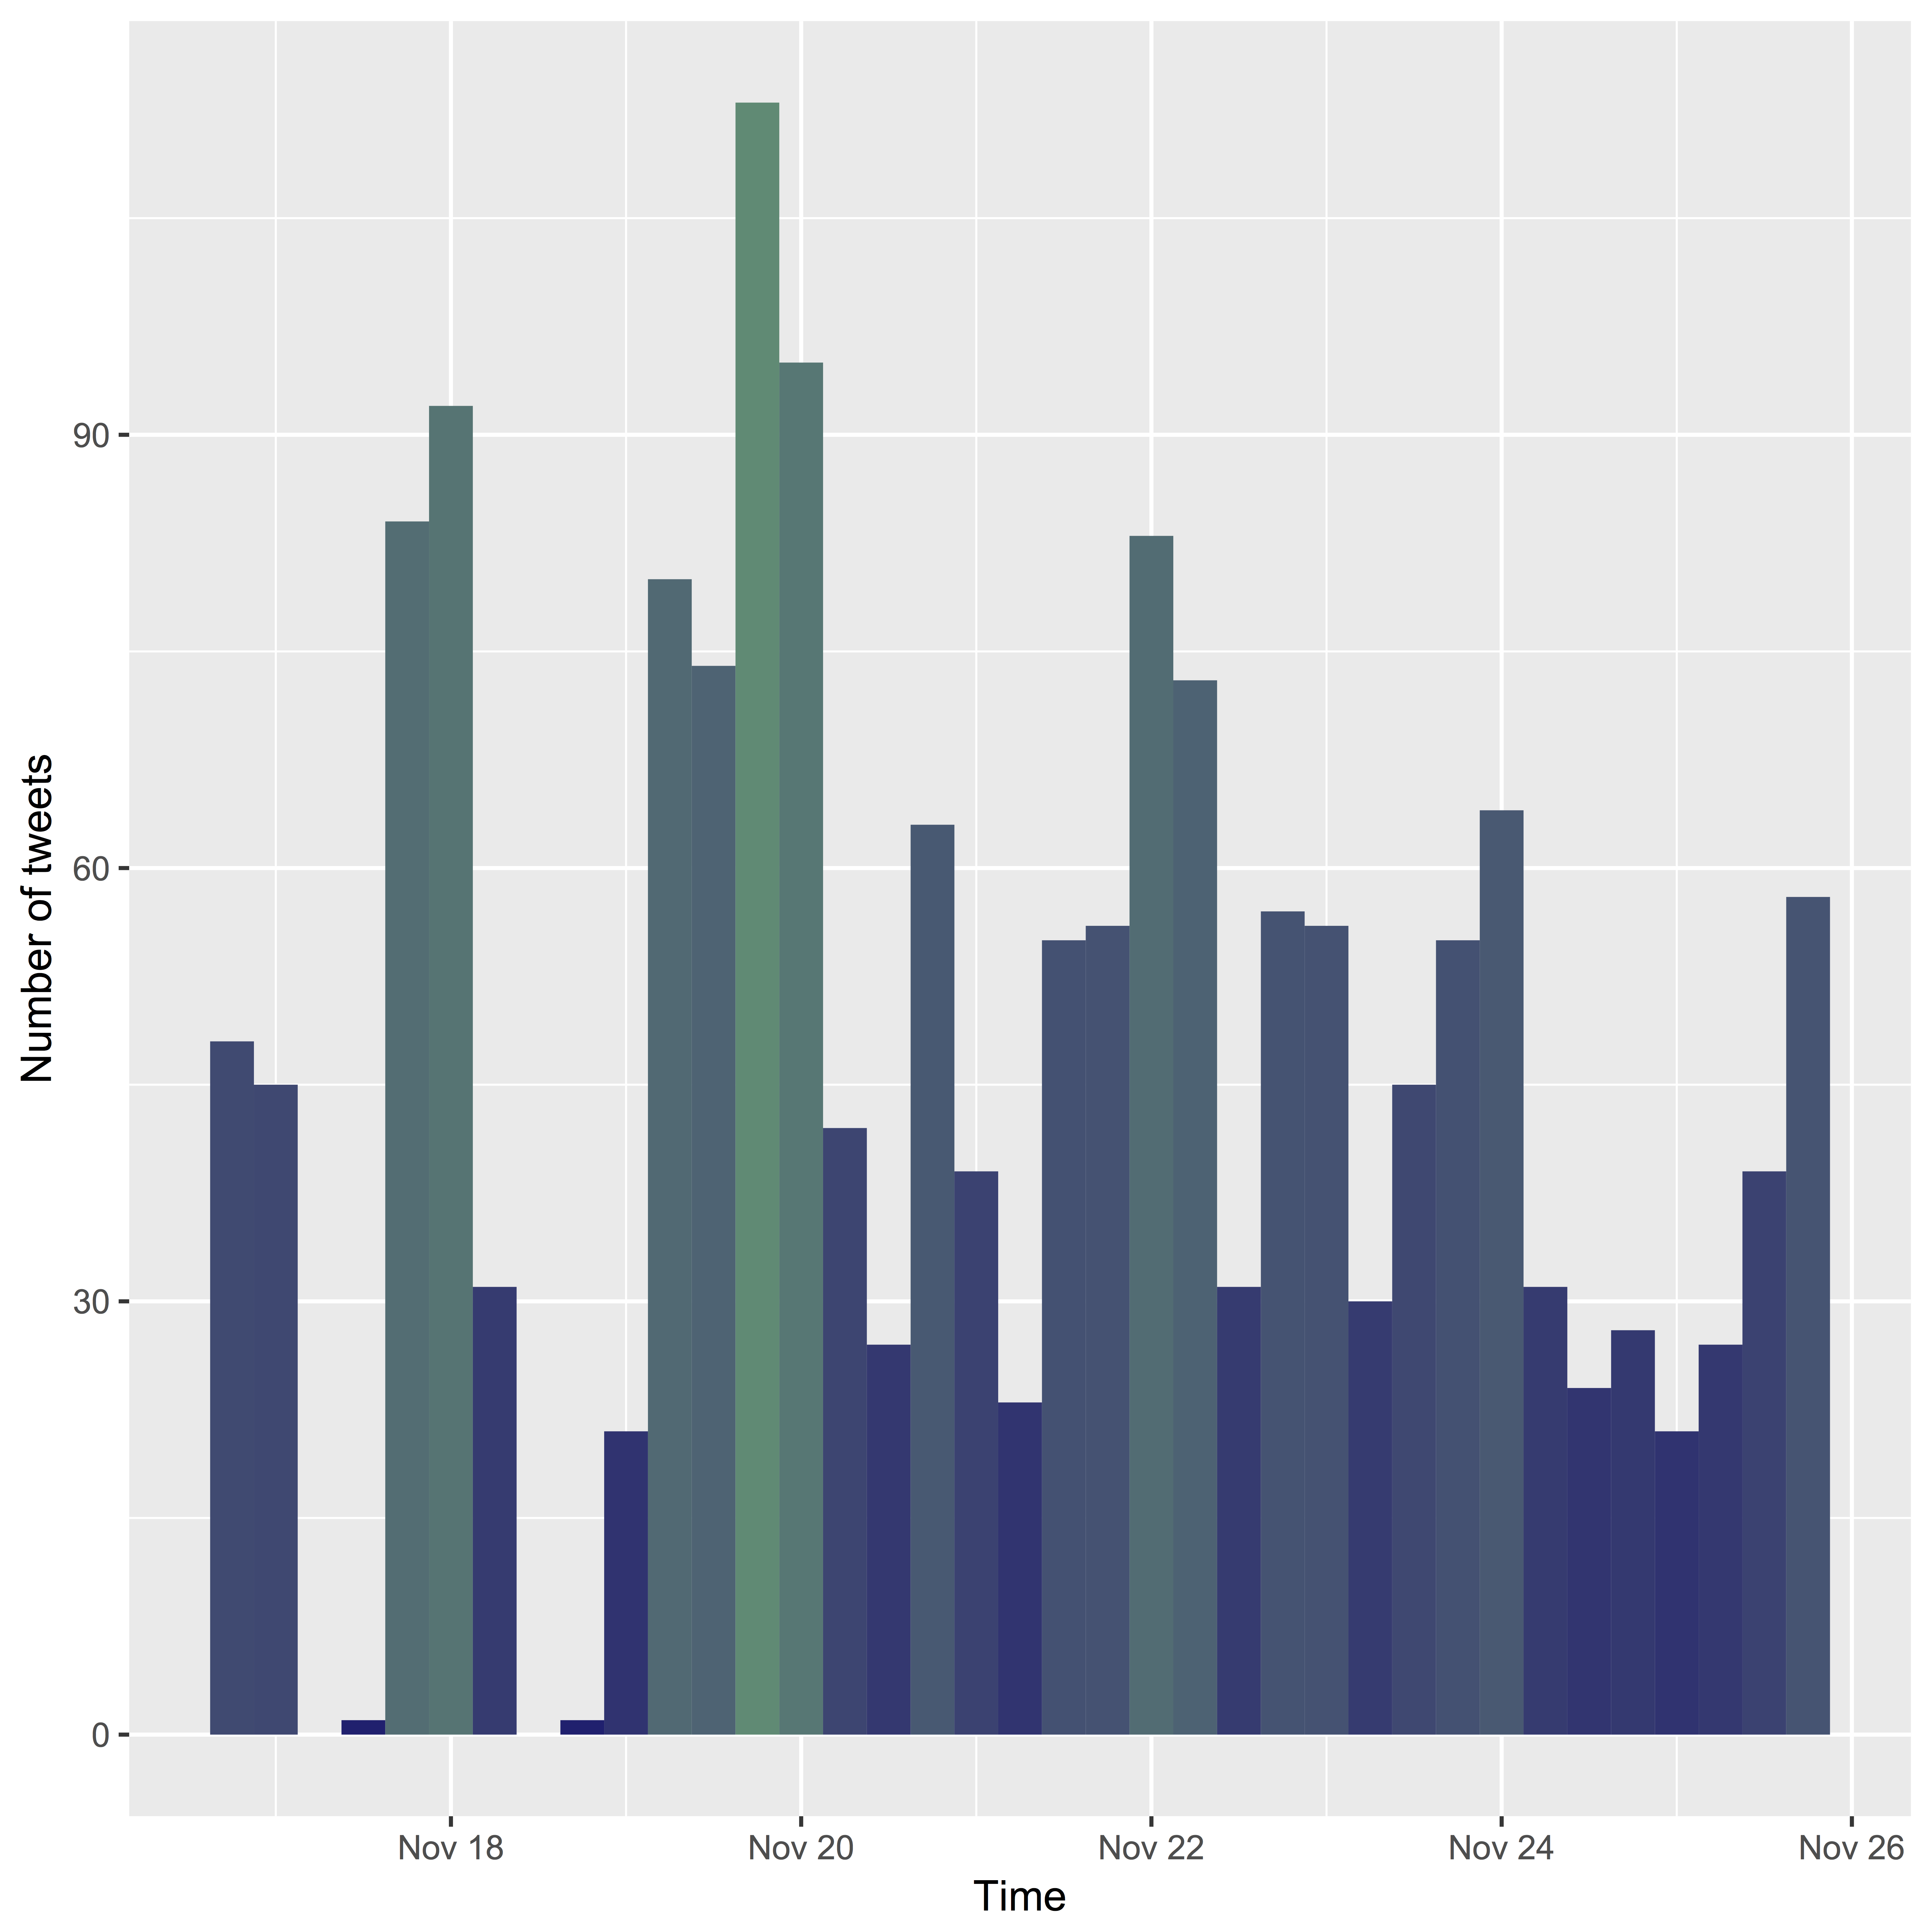
\includegraphics[height = 0.9\textheight]{eftfreq}
\end{frame}

\begin{frame}
	\frametitle{Number of Tweets Over Time (NotMyPresident)}
  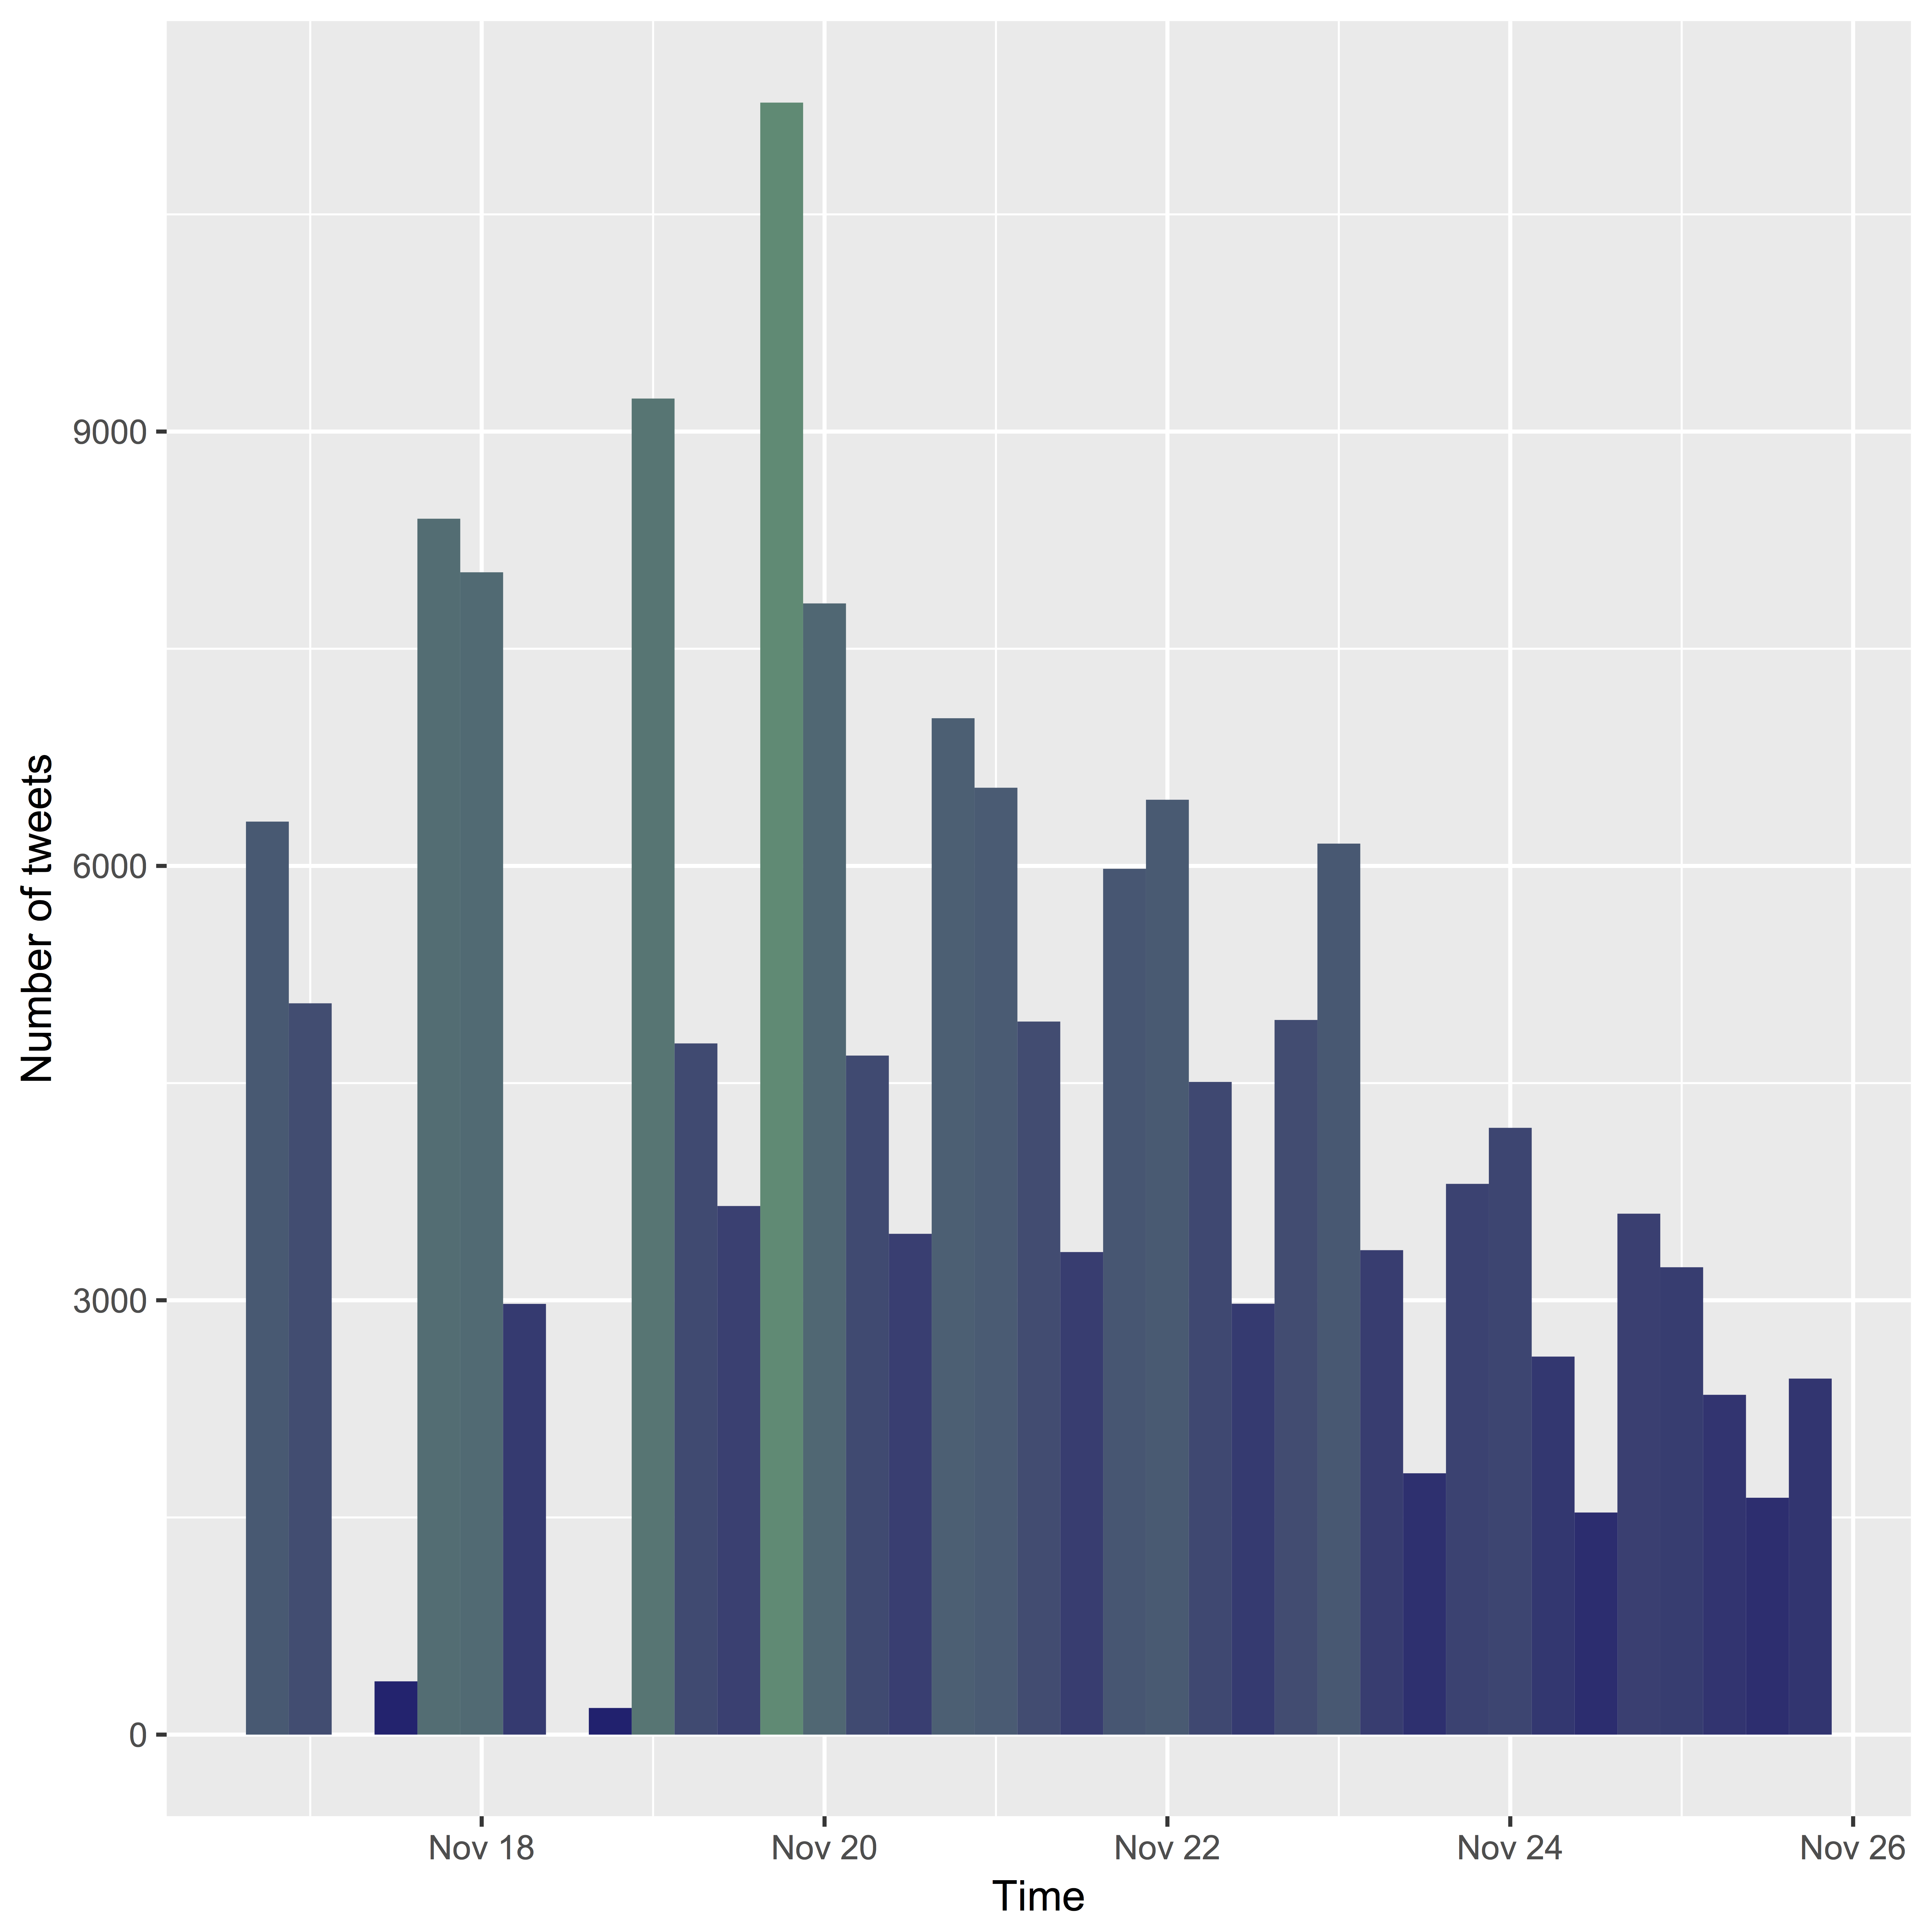
\includegraphics[height = 0.9\textheight]{nmpfreq}
\end{frame}

\begin{frame}
	\frametitle{Sentiments Over Time (Election2016)}
  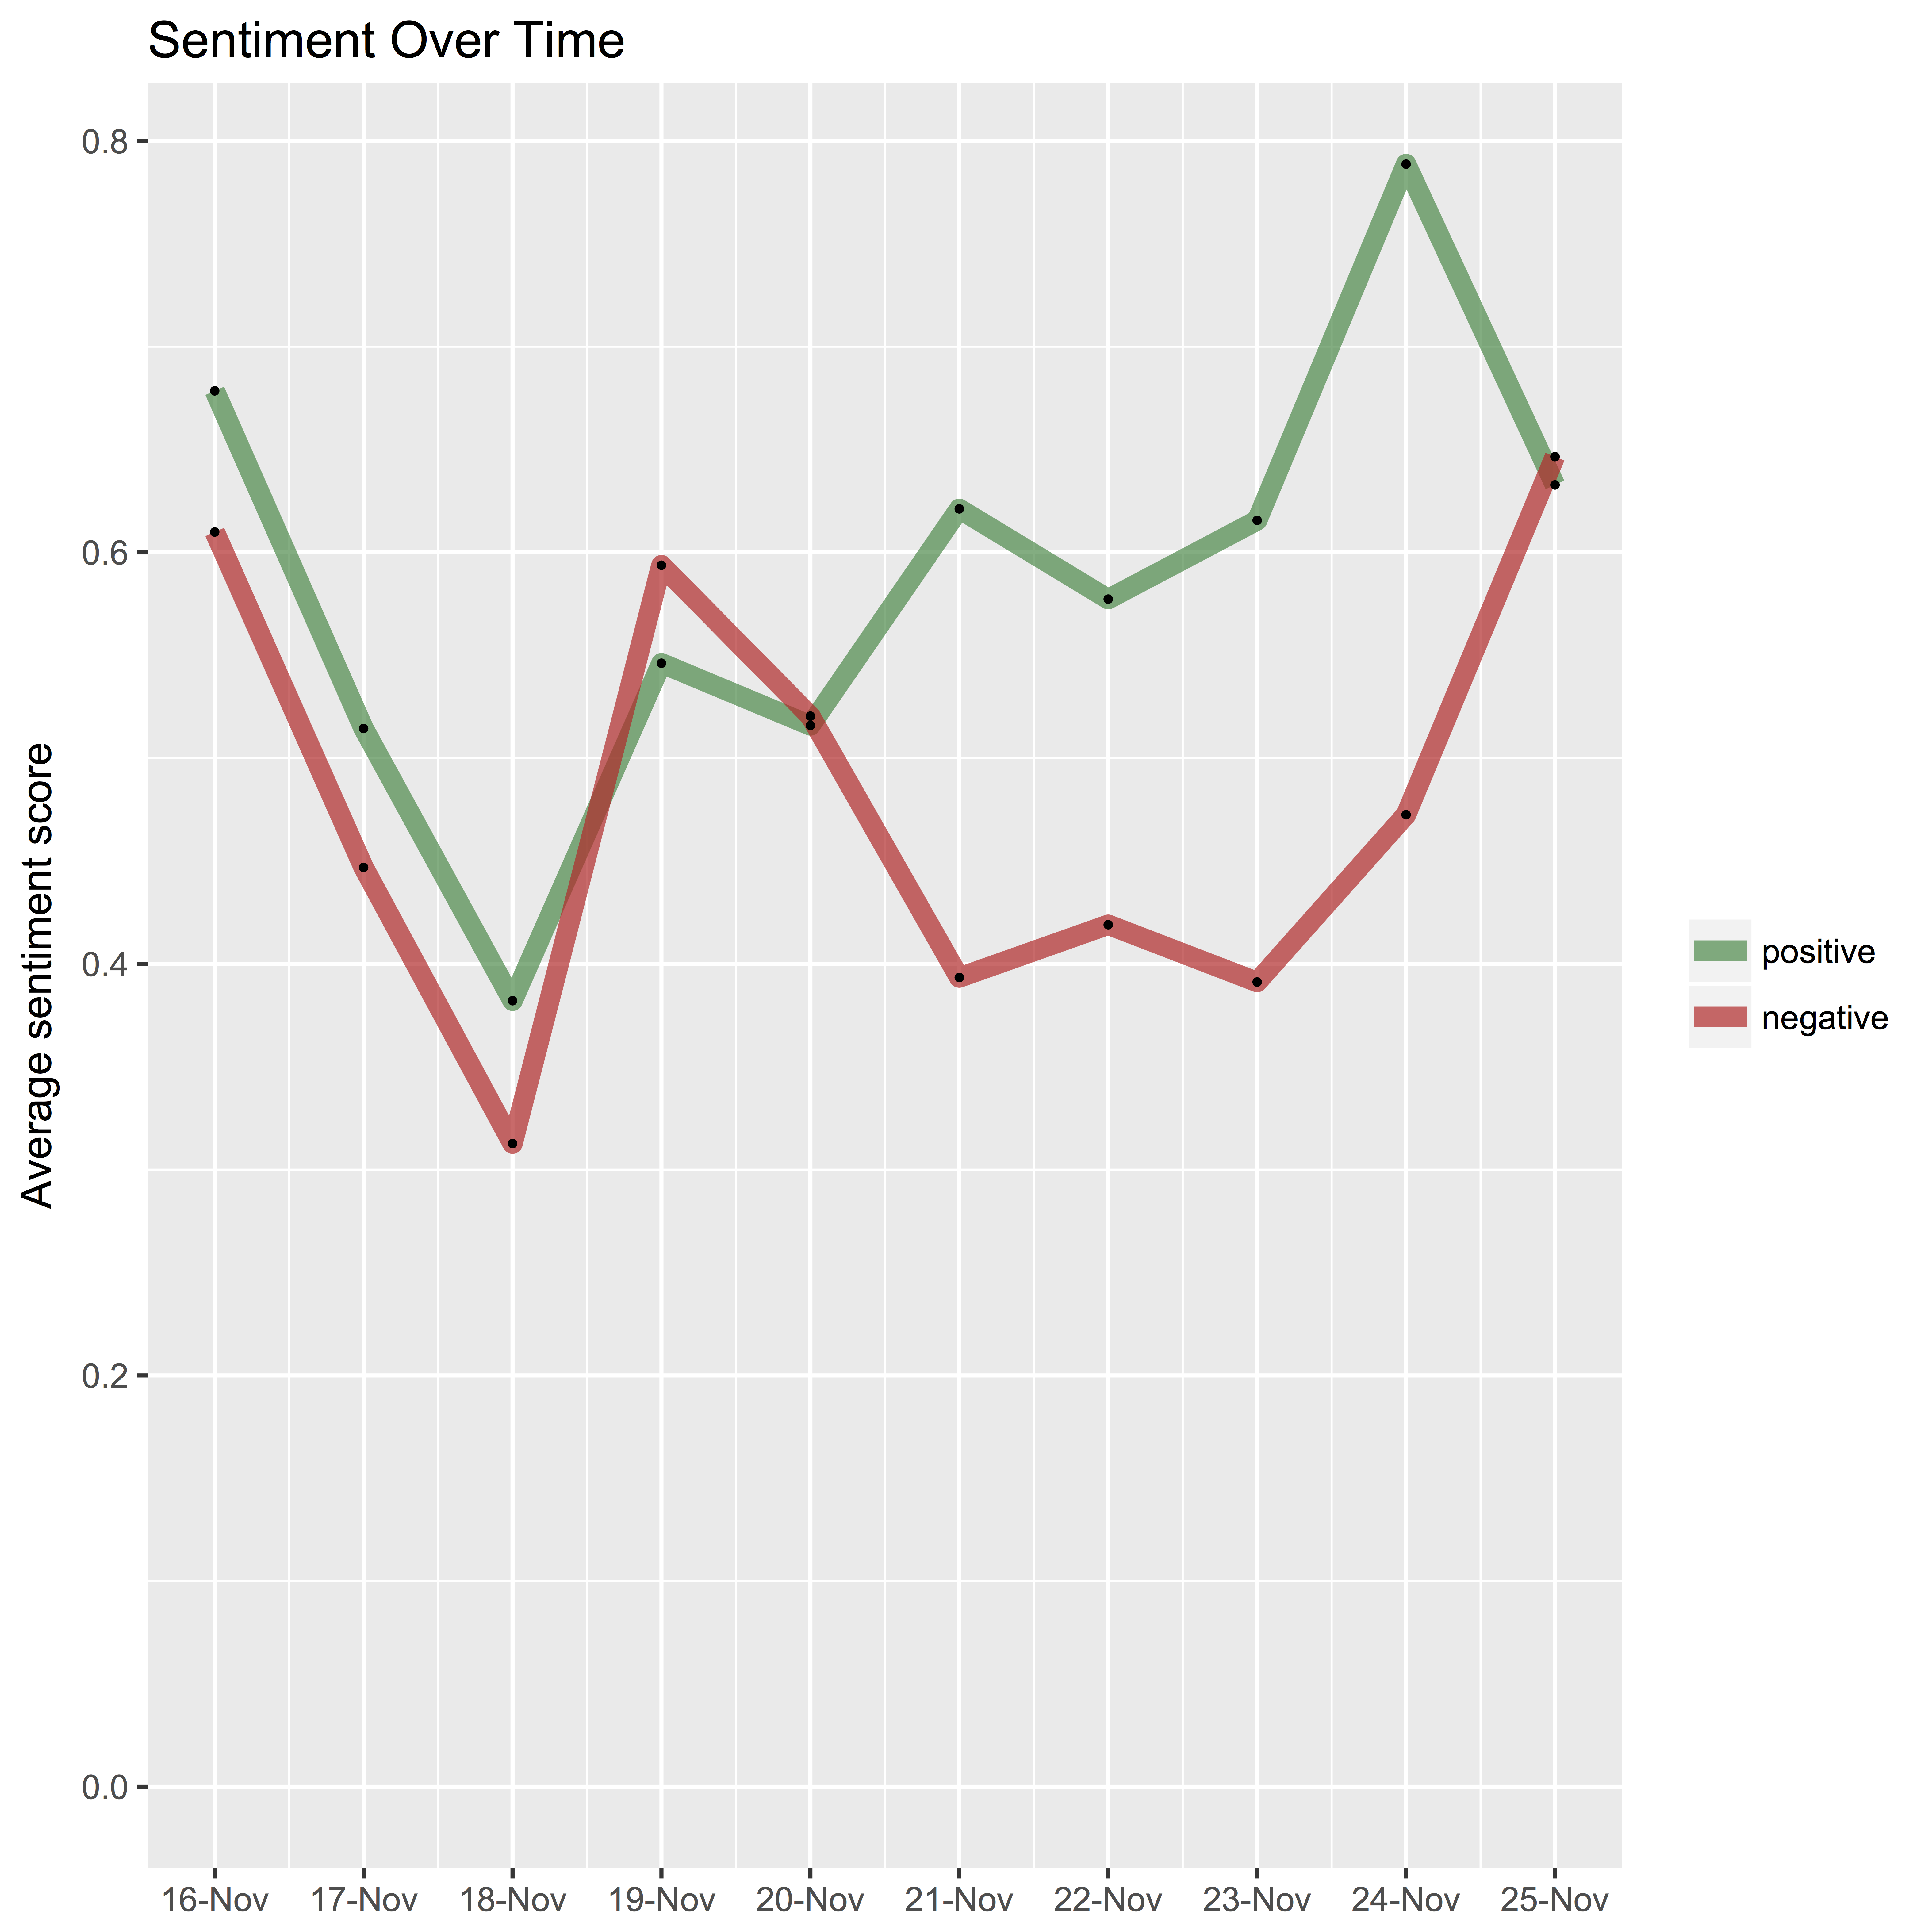
\includegraphics[height = 0.9\textheight]{e2016sentiments}
\end{frame}

\begin{frame}
	\frametitle{Sentiments Over Time (ElectionNight)}
  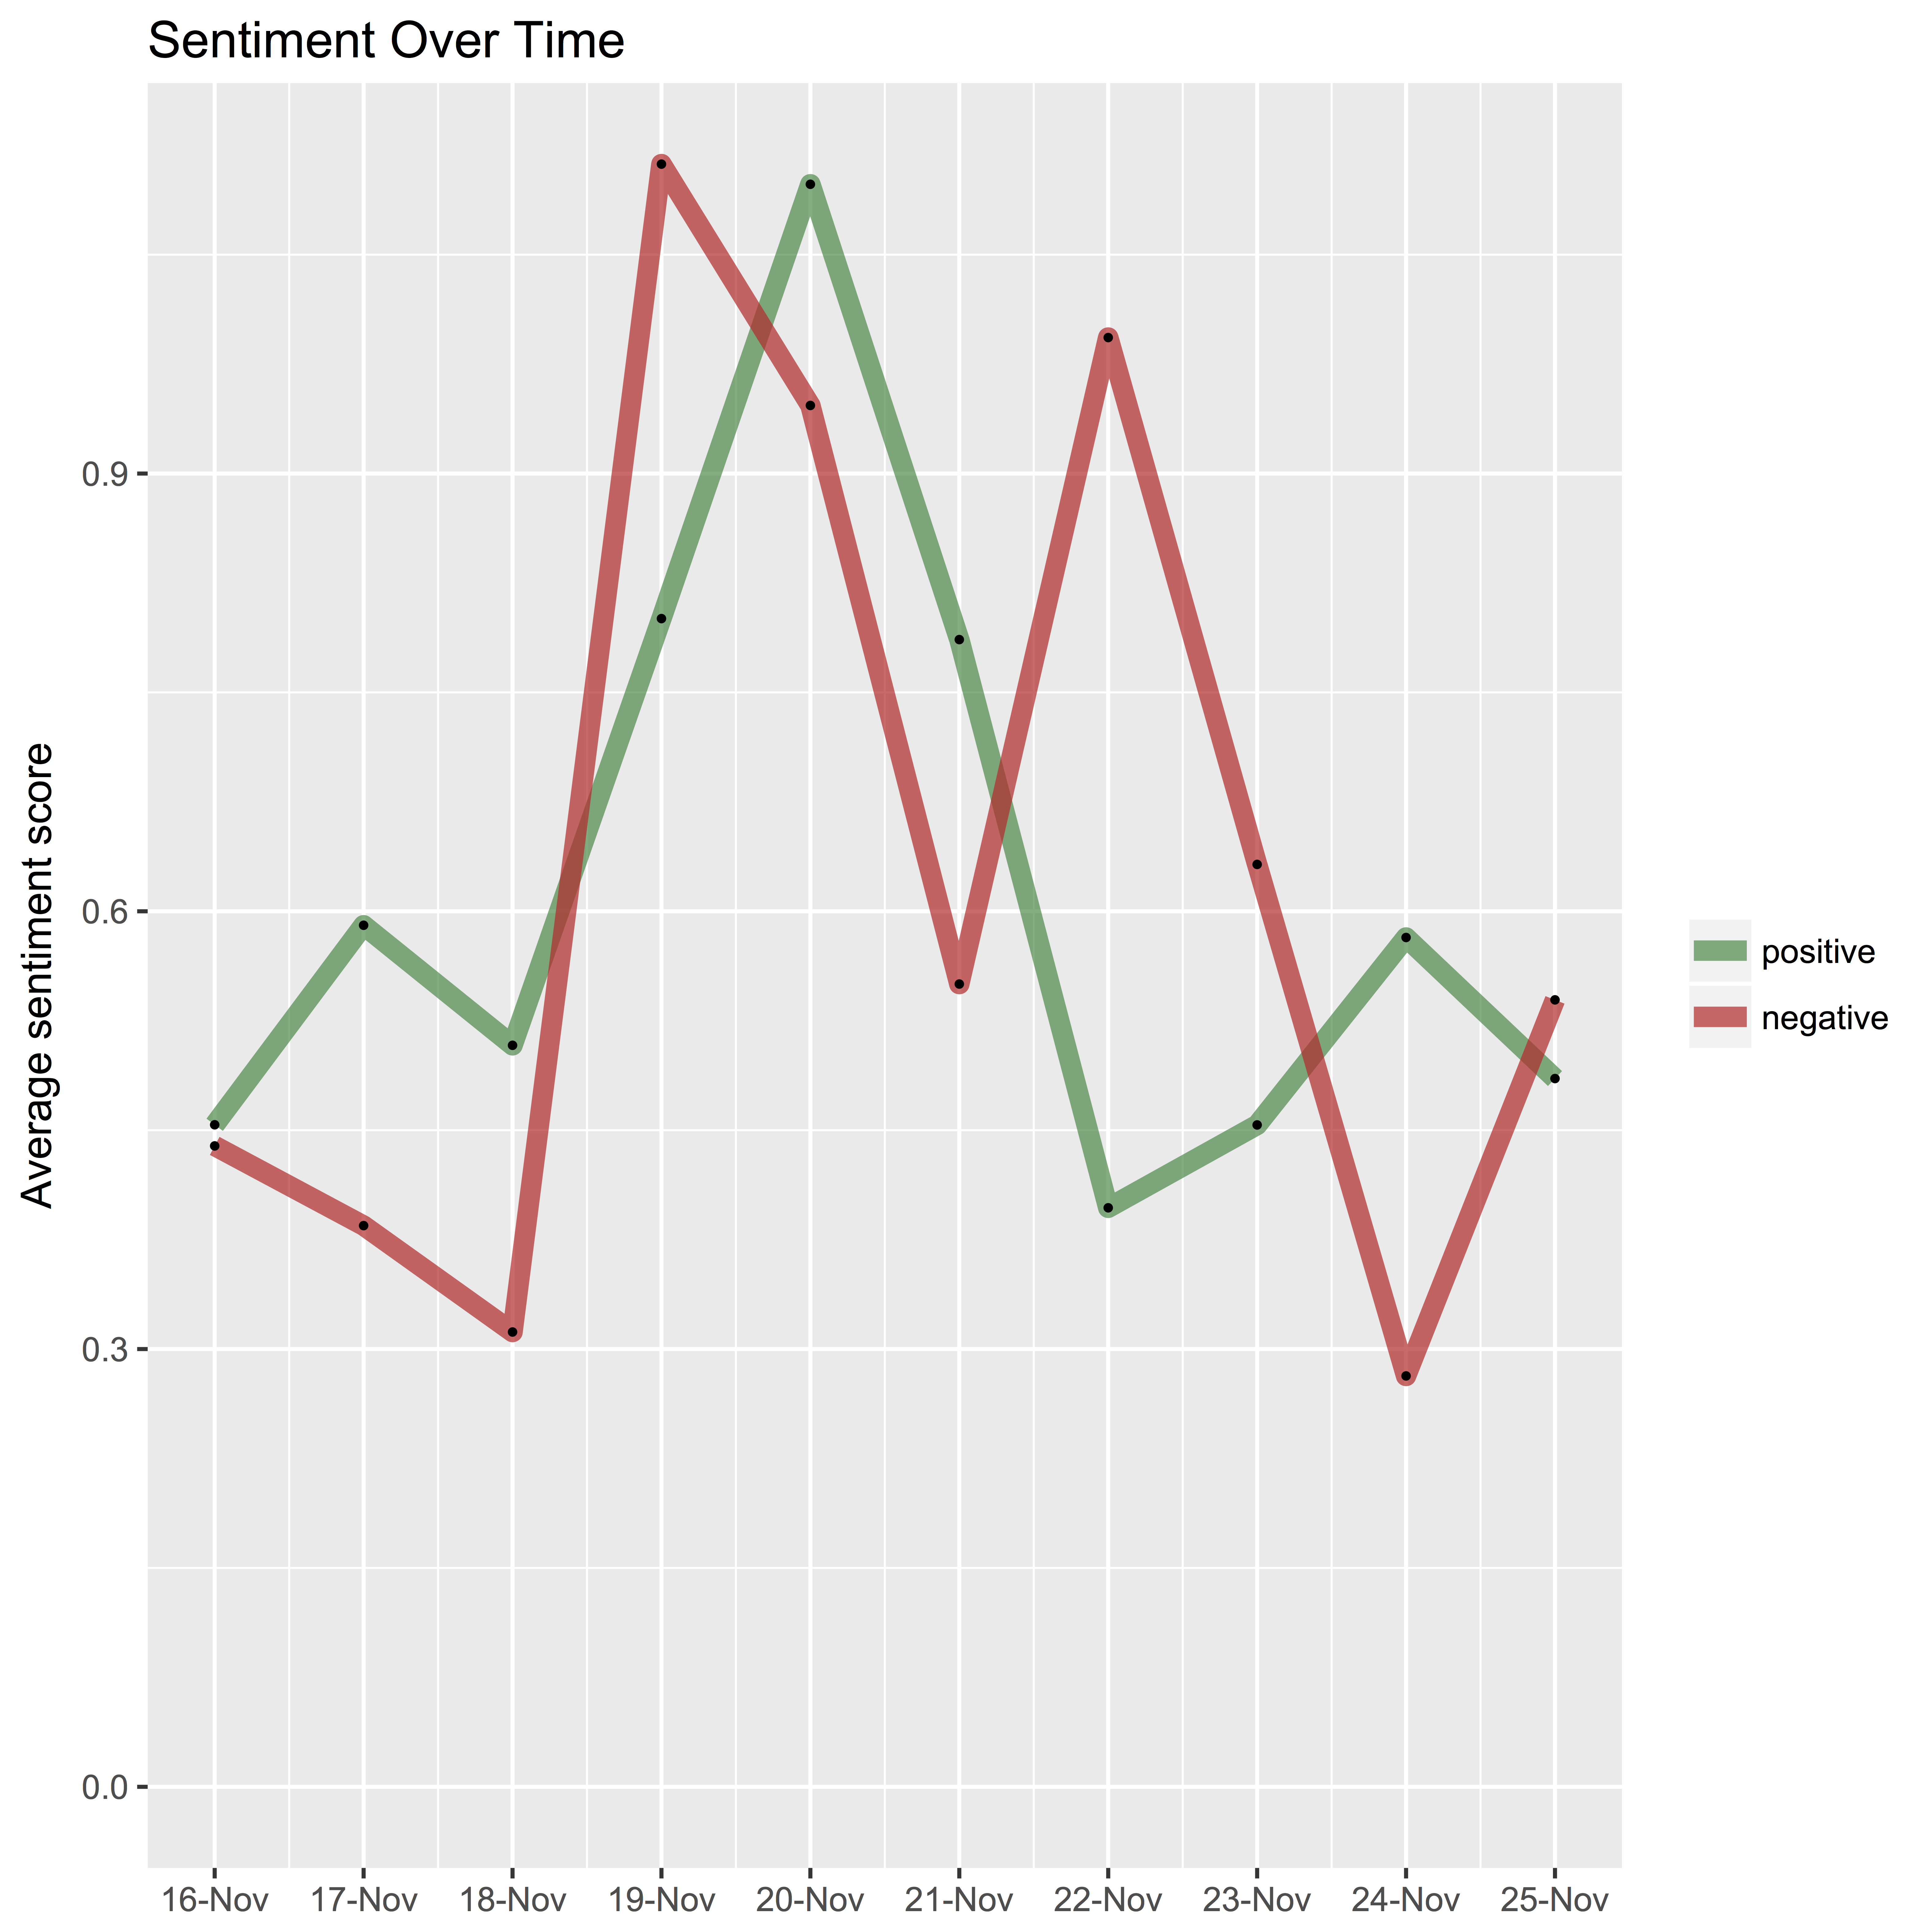
\includegraphics[height = 0.9\textheight]{ensentiments}
\end{frame}

\begin{frame}
	\frametitle{Sentiments Over Time (ElectionFinalThoughts)}
  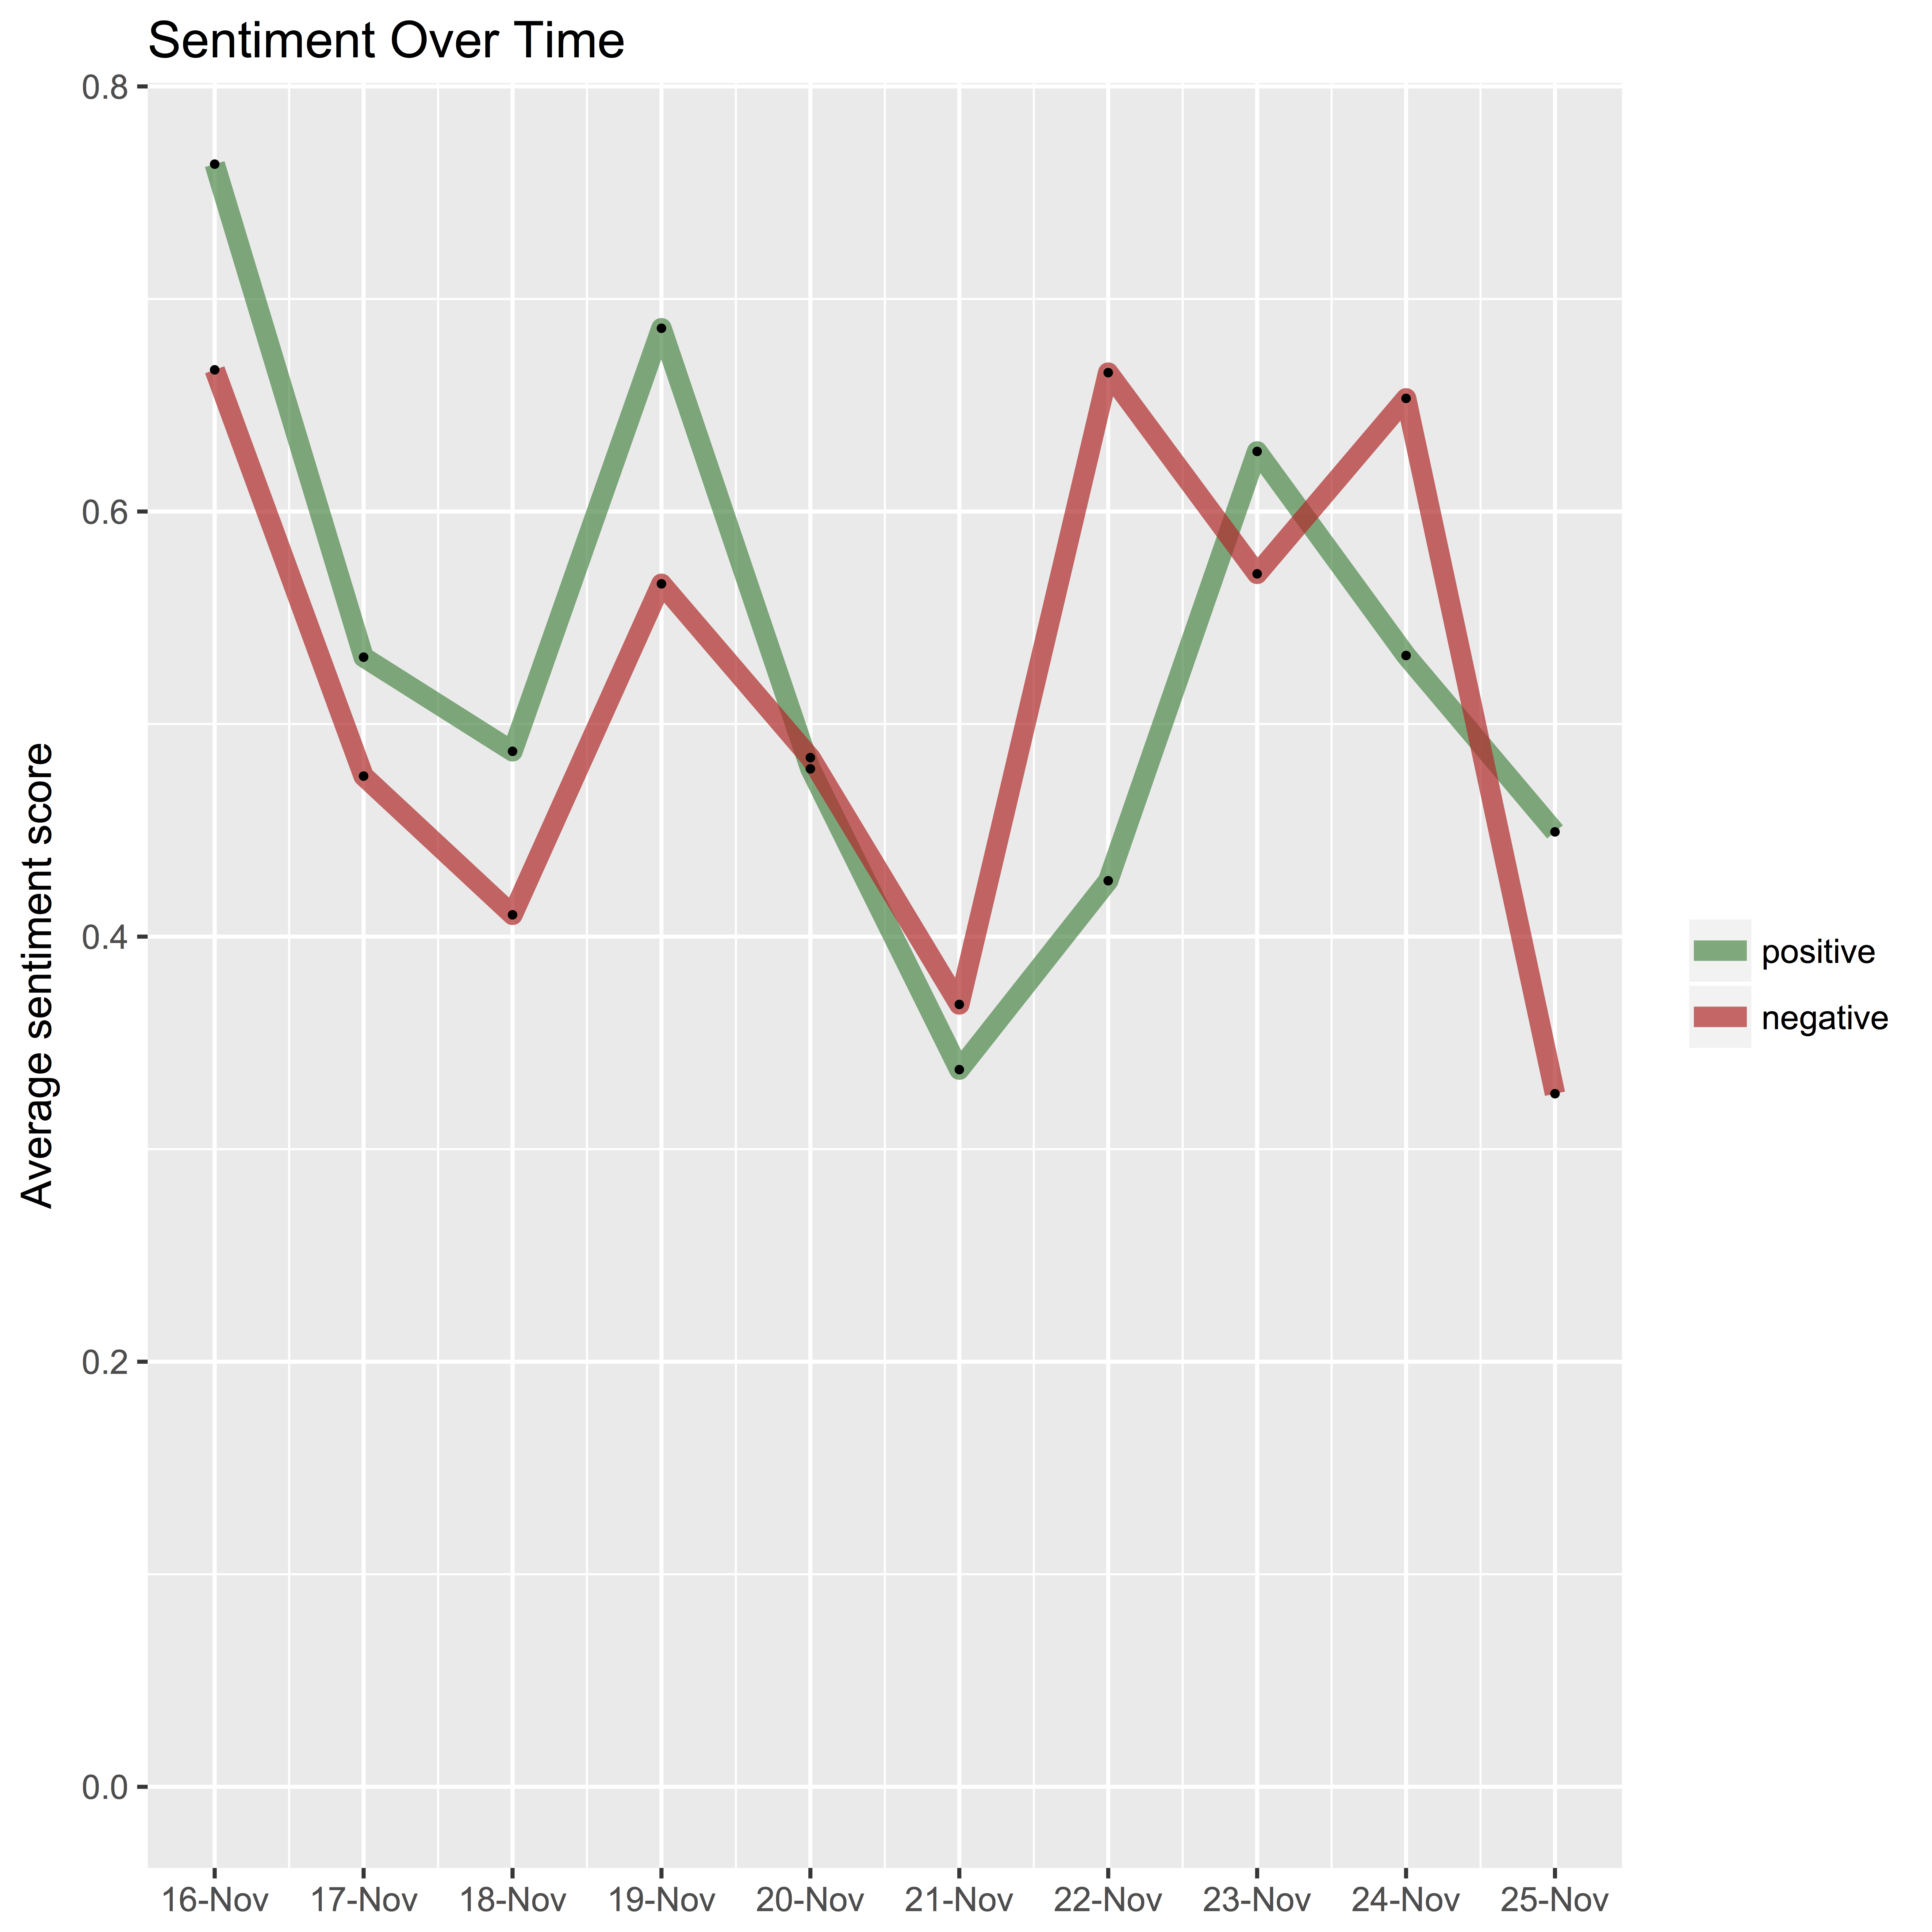
\includegraphics[height = 0.9\textheight]{eftsentiments}
\end{frame}

\begin{frame}
	\frametitle{Sentiments Over Time (NotMyPresident)}
  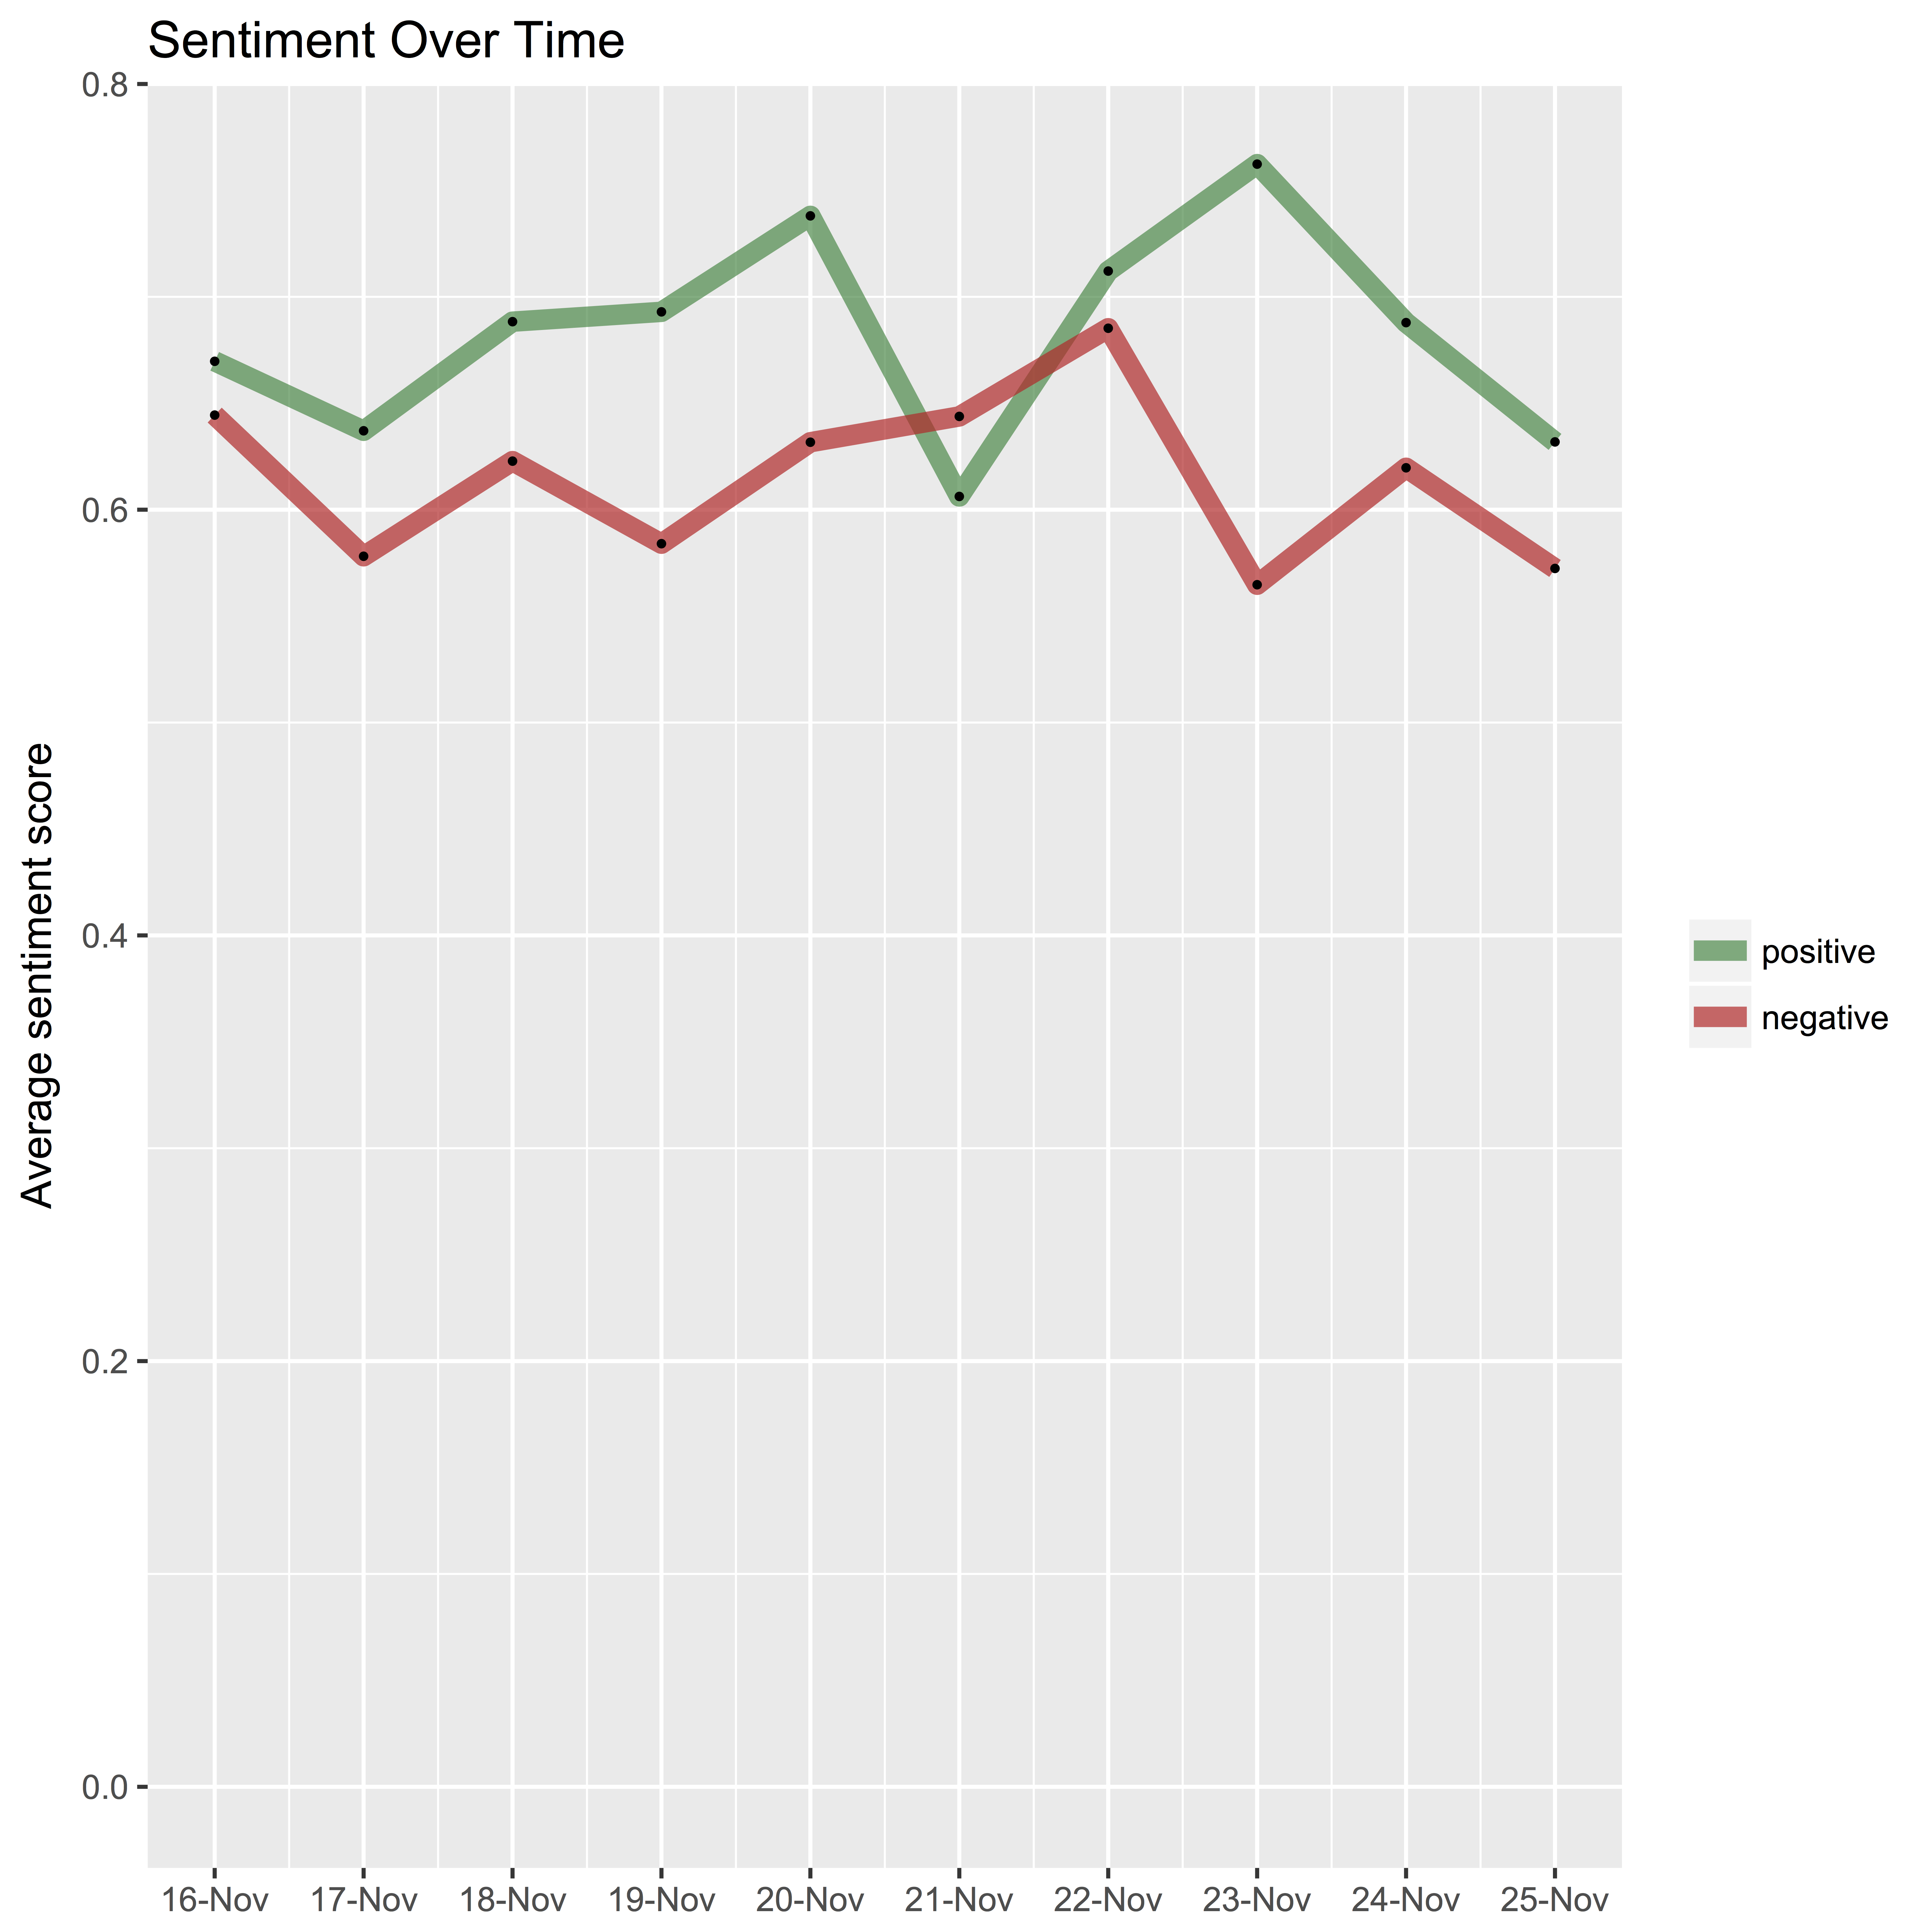
\includegraphics[height = 0.9\textheight]{nmpsentiments}
\end{frame}

\begin{frame}
	\frametitle{Map of Hashtags (Election2016)}
  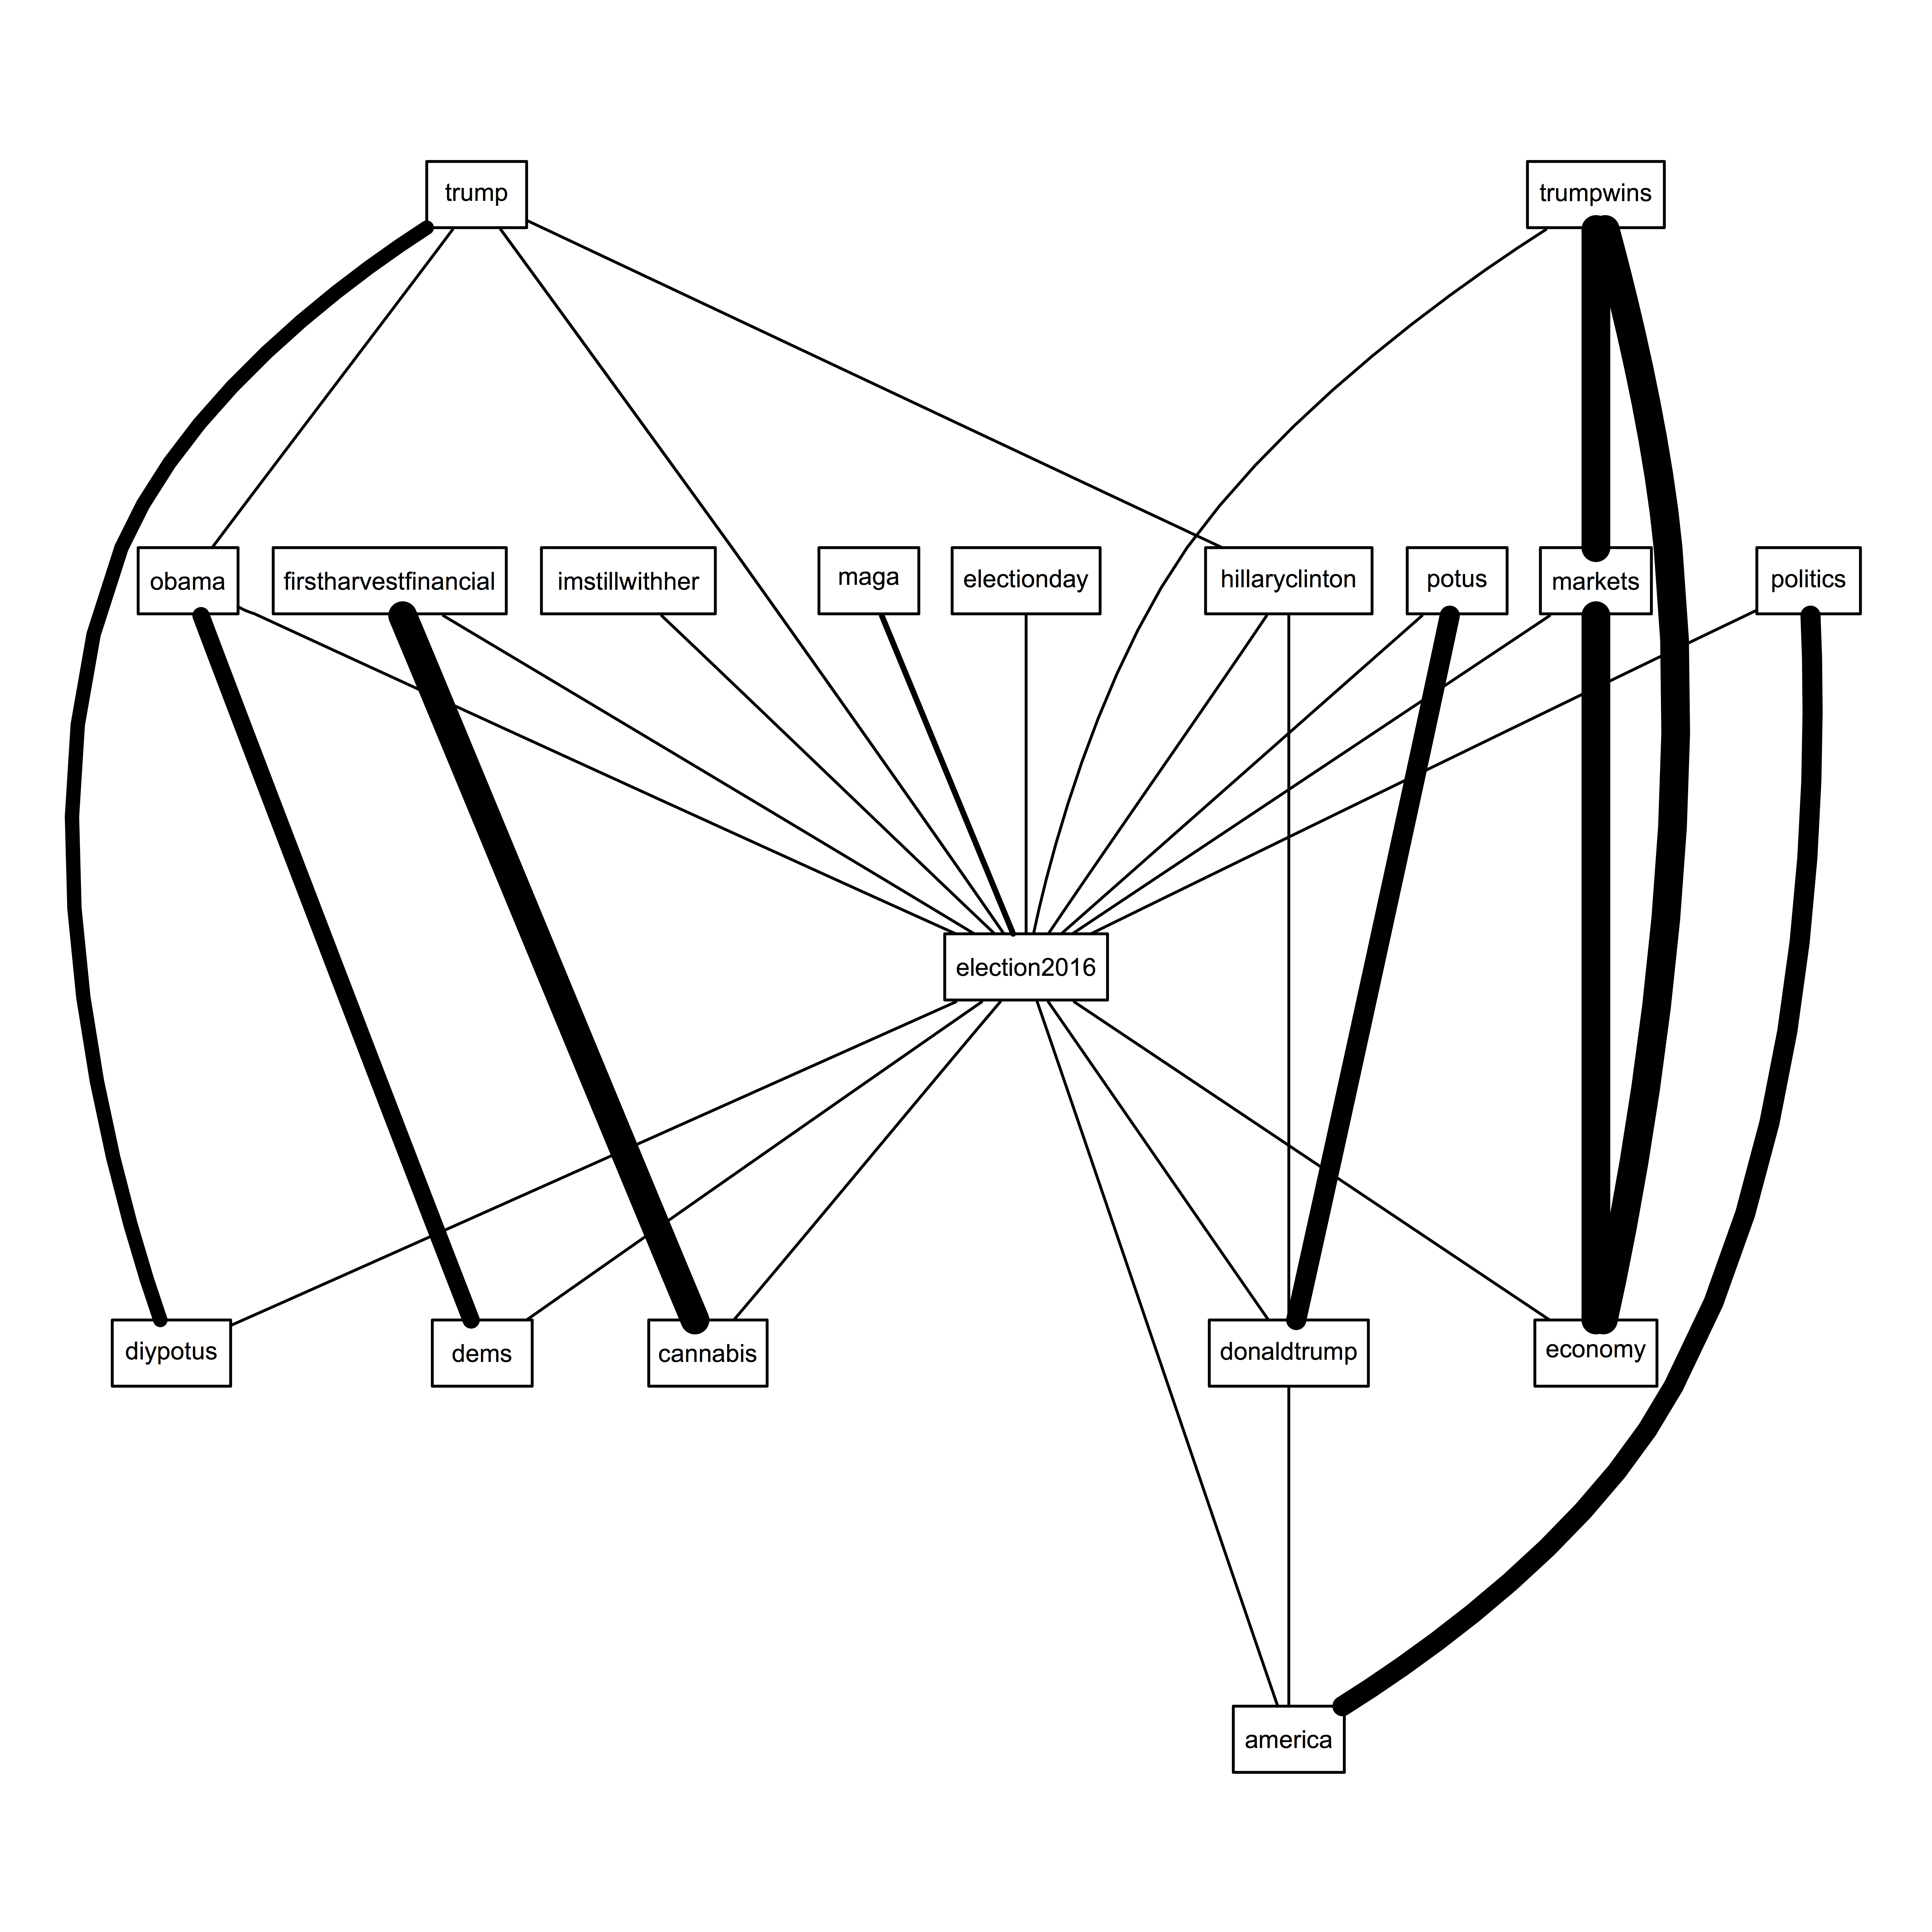
\includegraphics[height = 0.9\textheight]{e2016hashmap}
\end{frame}

\begin{frame}
	\frametitle{Map of Hashtags (NotMyPresident)}
  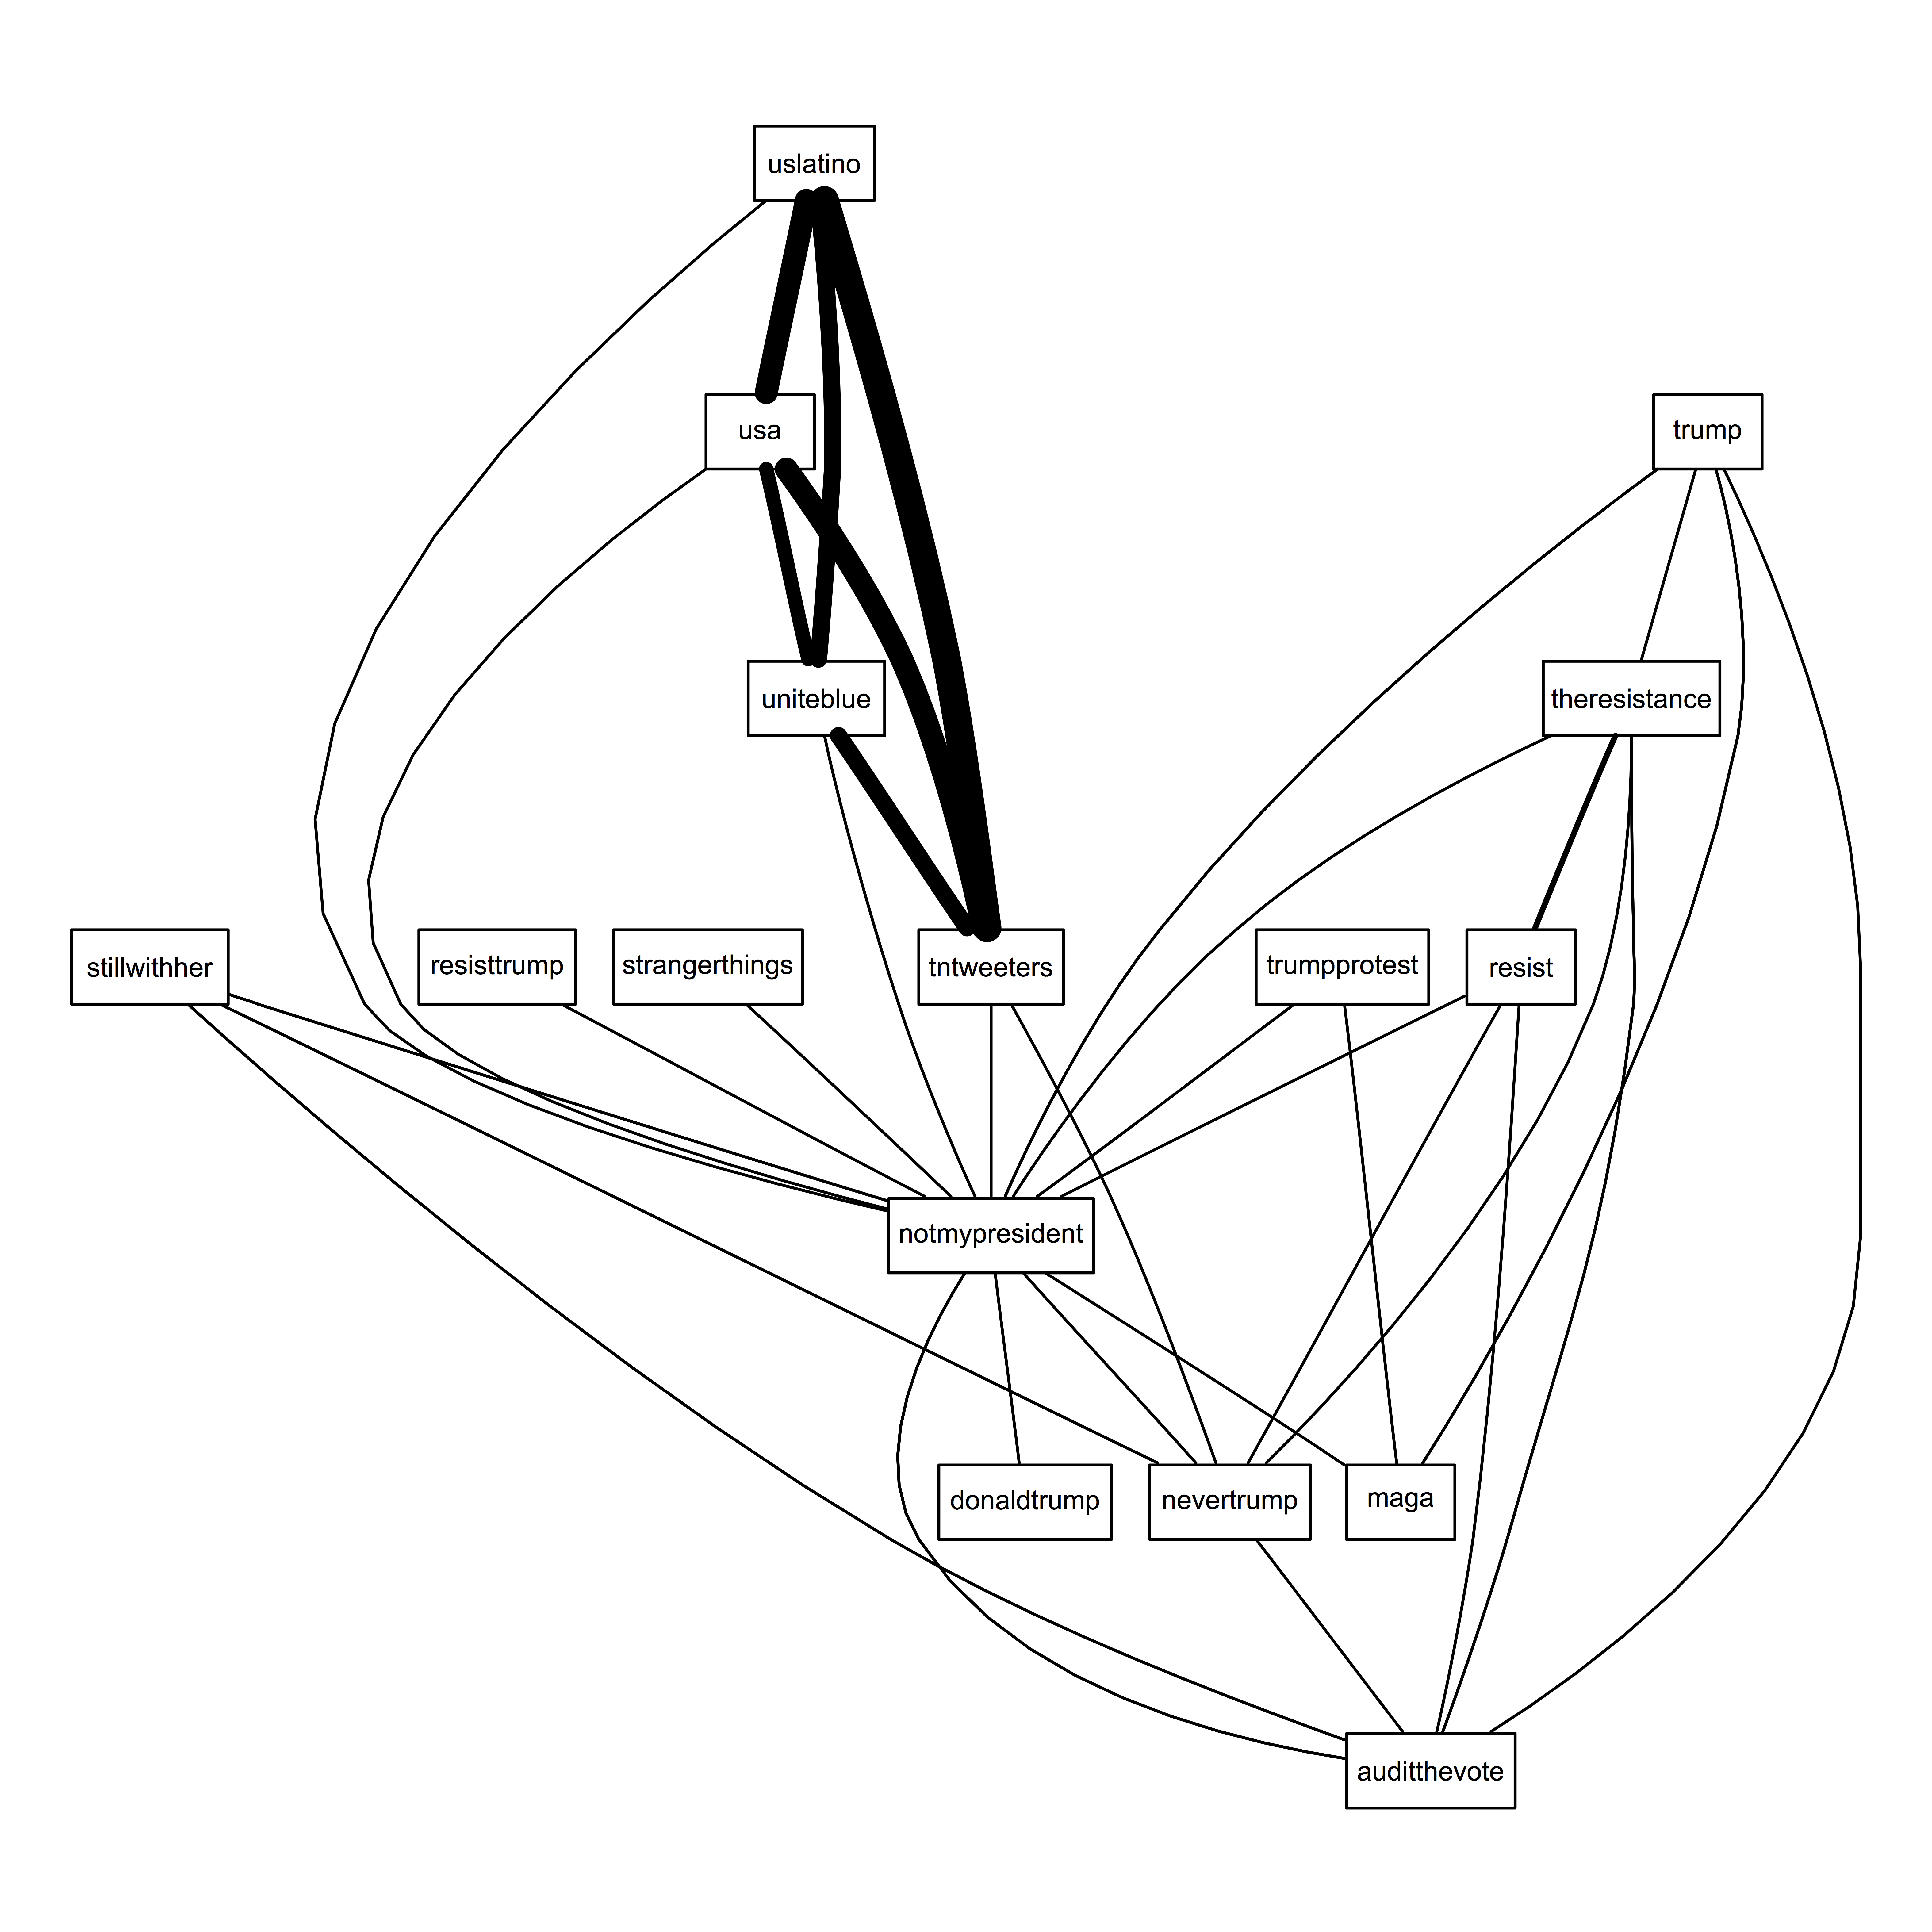
\includegraphics[height = 0.9\textheight]{nmphashmap}
\end{frame}

\begin{frame}
	\frametitle{Frequency of Hashtags (Election2016)}
  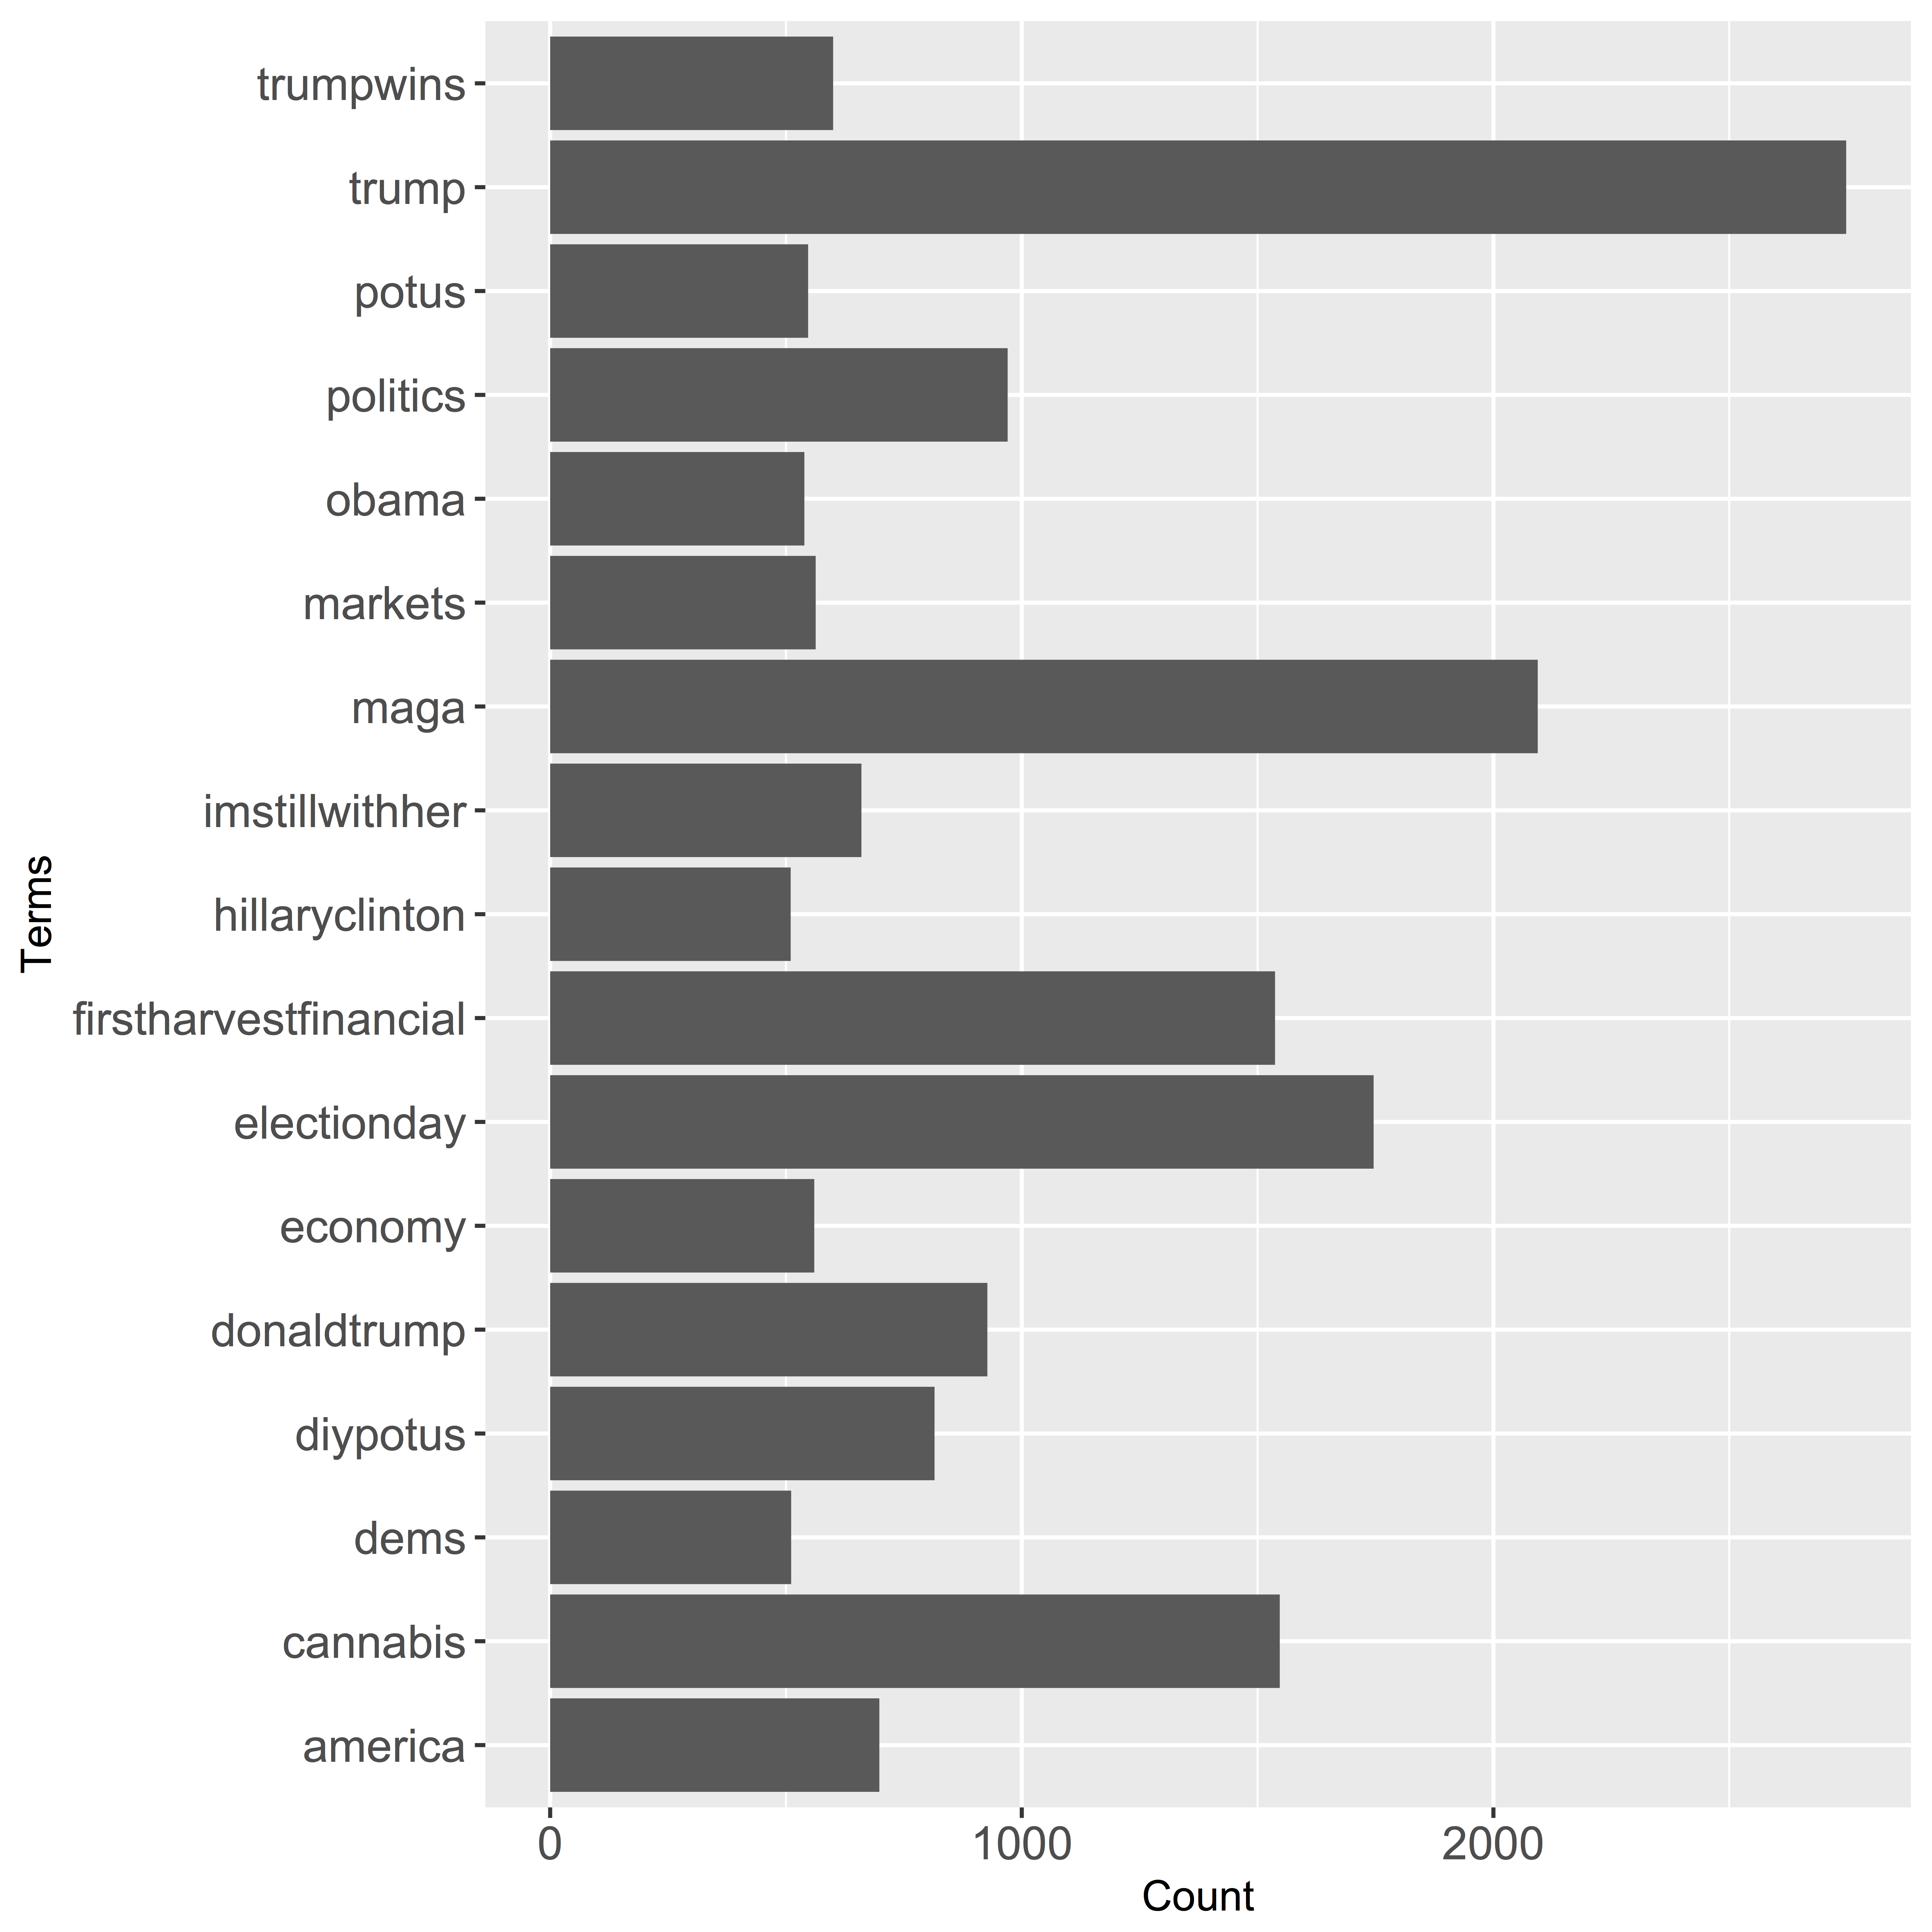
\includegraphics[height = 0.9\textheight]{e2016hashcount}
\end{frame}

\begin{frame}
	\frametitle{Frequency of Hashtags (NotMyPresident)}
  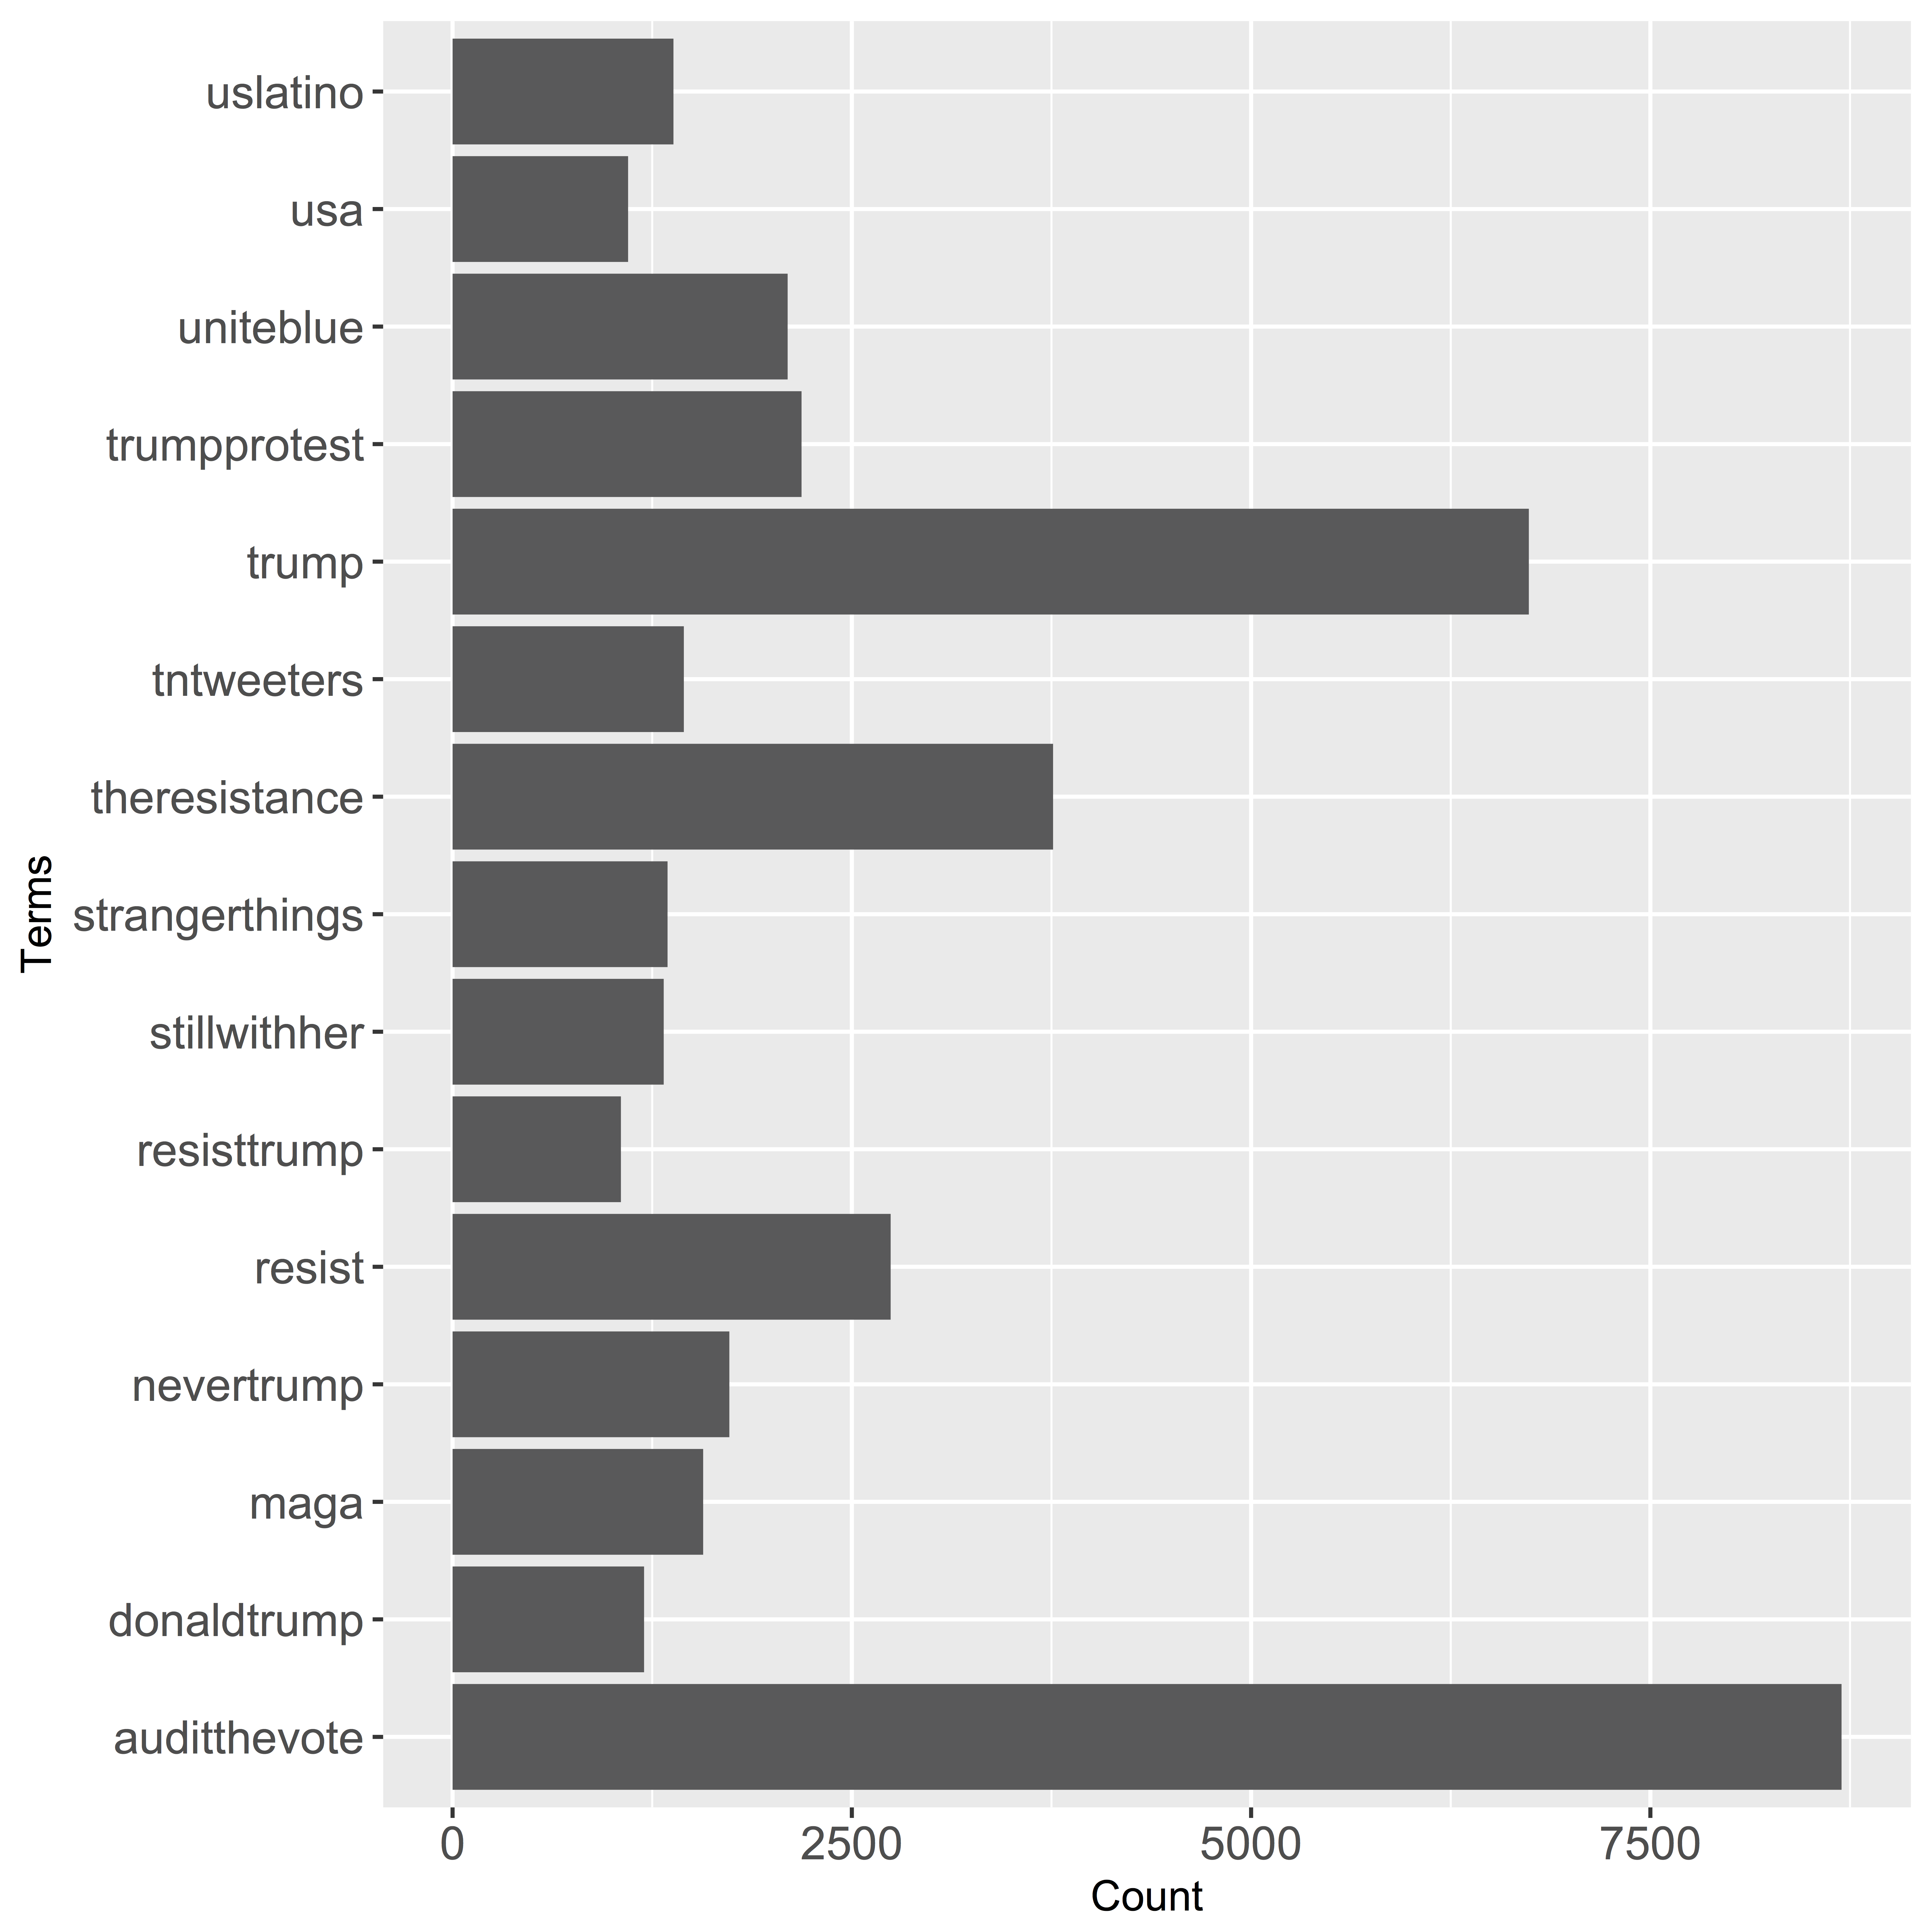
\includegraphics[height = 0.9\textheight]{nmphashcount}
\end{frame}

\begin{frame}
	\frametitle{Frequency of Emoji (Election2016)}
  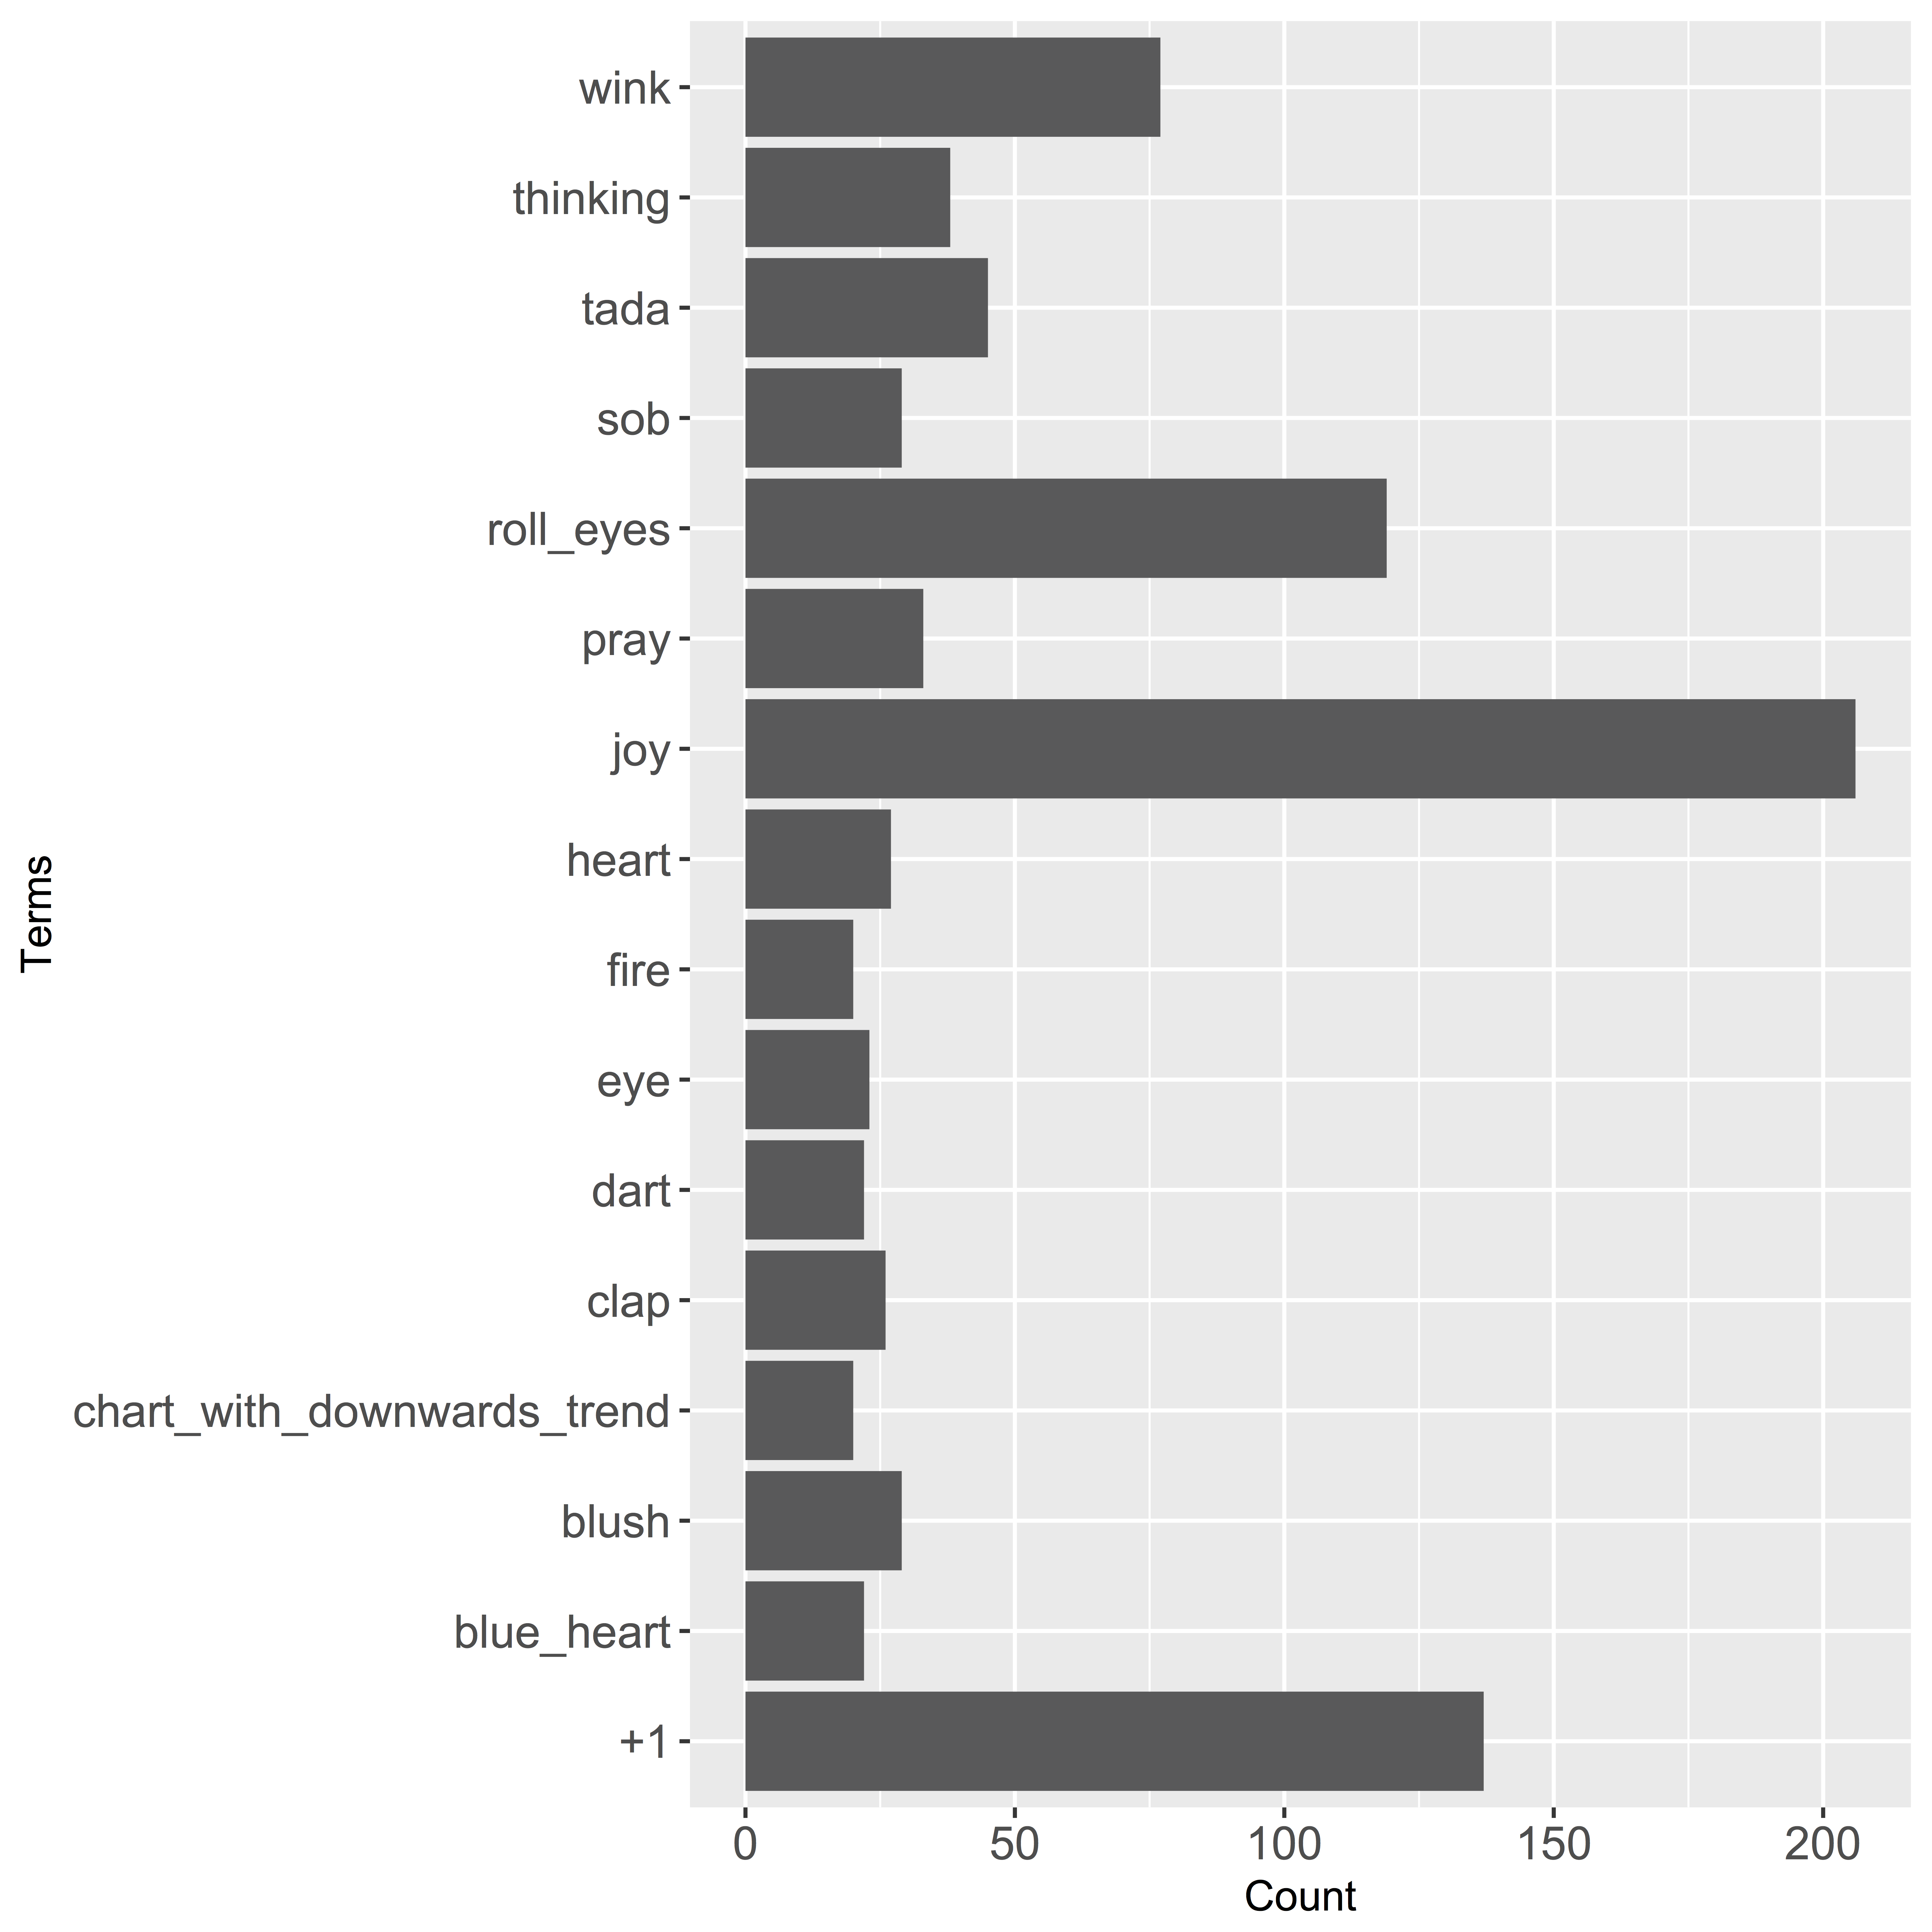
\includegraphics[height = 0.9\textheight]{e2016emoji}
\end{frame}

\begin{frame}
	\frametitle{Frequency of Emoji (NotMyPresident)}
  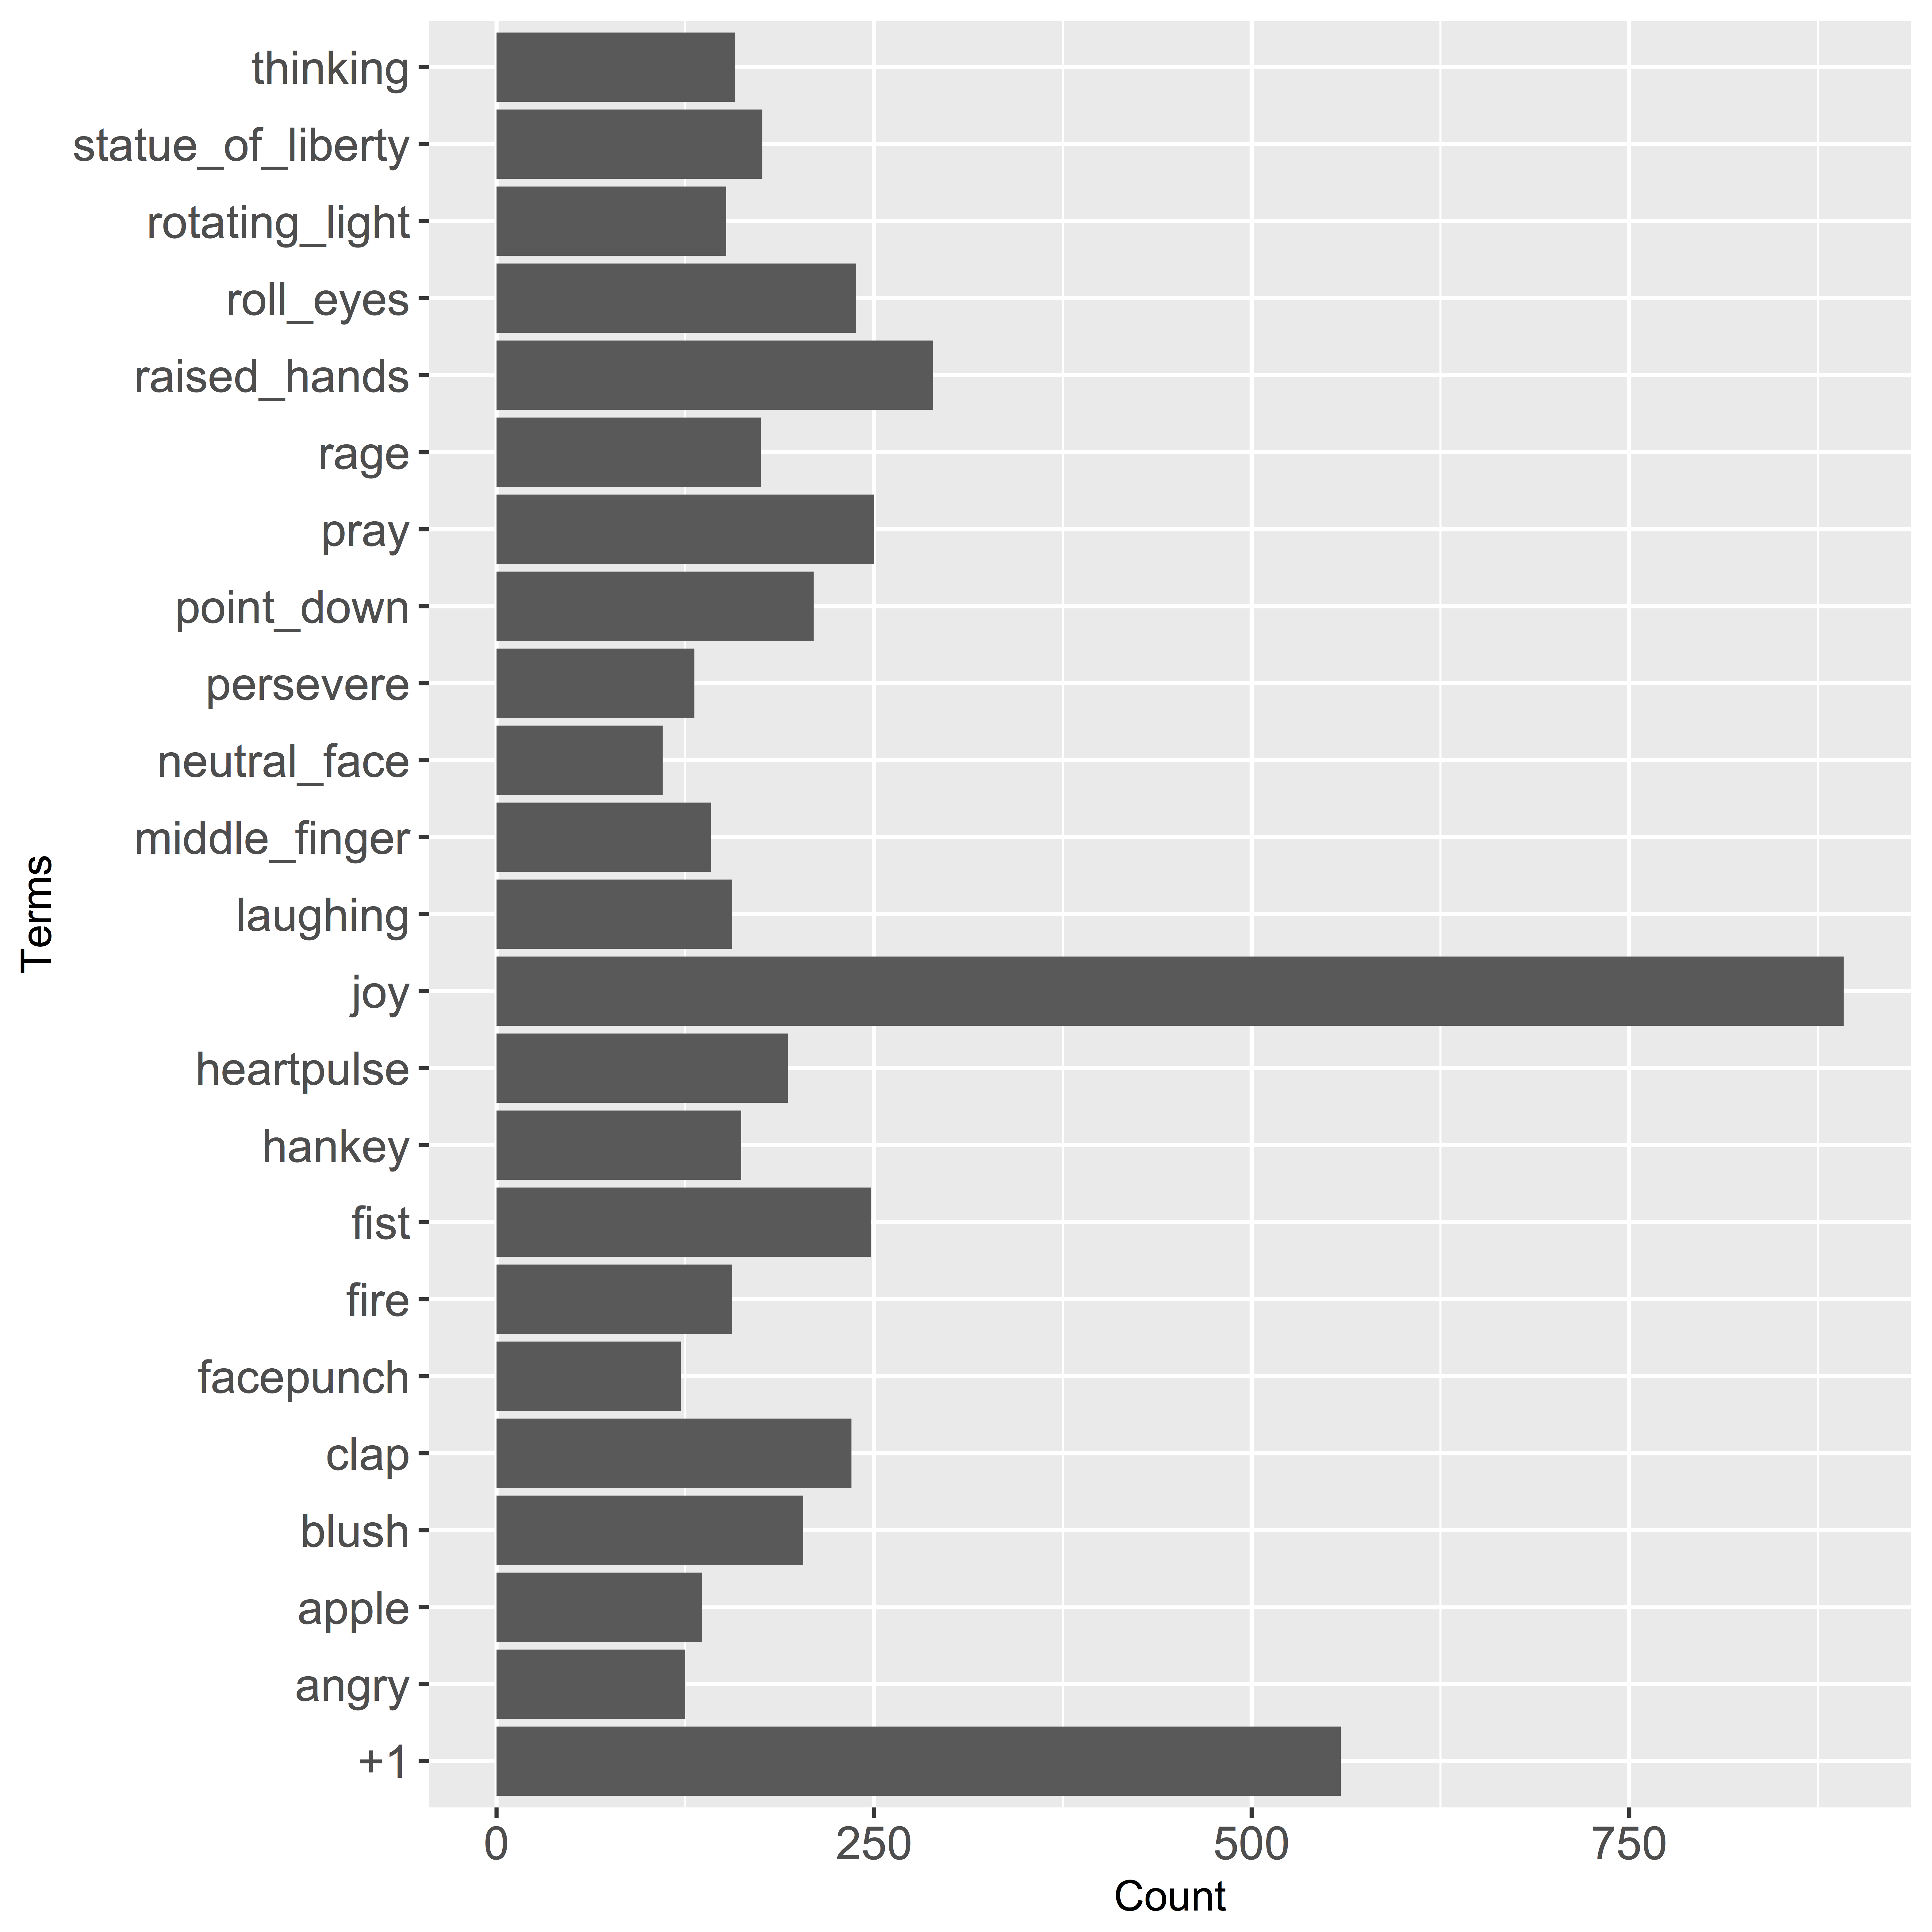
\includegraphics[height = 0.9\textheight]{nmpemoji}
\end{frame}

%----------------------------------------------------------------------------------------

\end{document} 